%%%%%%%%%%%%%%%%%%%%%%%%%%%%%%%%%%%%%%%%%%%%%%%%%%%%%%%%%%%%%%%%%%%%%%%%%%%%%%%%
%
% Template license:
% CC BY-NC-SA 3.0 (http://creativecommons.org/licenses/by-nc-sa/3.0/)
%
%%%%%%%%%%%%%%%%%%%%%%%%%%%%%%%%%%%%%%%%%%%%%%%%%%%%%%%%%%%%%%%%%%%%%%%%%%%%%%%%

%----------------------------------------------------------------------------------------
%	PACKAGES AND OTHER DOCUMENT CONFIGURATIONS
%----------------------------------------------------------------------------------------

\documentclass[
11pt, % The default document font size, options: 10pt, 11pt, 12pt
%oneside, % Two side (alternating margins) for binding by default, uncomment to switch to one side
%chapterinoneline,% Have the chapter title next to the number in one single line
spanish,
singlespacing, % Single line spacing, alternatives: onehalfspacing or doublespacing
%draft, % Uncomment to enable draft mode (no pictures, no links, overfull hboxes indicated)
%nolistspacing, % If the document is onehalfspacing or doublespacing, uncomment this to set spacing in lists to single
%liststotoc, % Uncomment to add the list of figures/tables/etc to the table of contents
%toctotoc, % Uncomment to add the main table of contents to the table of contents
parskip, % Uncomment to add space between paragraphs
%codirector, % Uncomment to add a codirector to the title page
headsepline, % Uncomment to get a line under the header
]{MastersDoctoralThesis} % The class file specifying the document structure

%\counterwithout{footnote}{chapter}

%----------------------------------------------------------------------------------------
%	INFORMACIÓN DE LA MEMORIA
%----------------------------------------------------------------------------------------

\thesistitle{Controlador CAN de servomotores} % El títulos de la memoria, se usa en la carátula y se puede usar el cualquier lugar del documento con el comando \ttitle

% Nombre del posgrado, se usa en la carátula y se puede usar el cualquier lugar del documento con el comando \degreename
\posgrado{Carrera de Especialización en Sistemas Embebidos} 

\author{Ing. Alejandro Virgillo} % Tu nombre, se usa en la carátula y se puede usar el cualquier lugar del documento con el comando \authorname

\director{Esp. Ing. Gabriel Gavinowich (FIUBA)} % El nombre del director, se usa en la carátula y se puede usar el cualquier lugar del documento con el comando \dirname
\codirector{Nombre del codirector (pertenencia)} % El nombre del codirector si lo hubiera, se usa en la carátula y se puede usar el cualquier lugar del documento con el comando \codirname.  Para activar este campo se debe descomentar la opción "codirector" en el comando \documentclass, línea 23.

\juradoUNO{Esp. Ing. Lic. Pablo José Carlos Alonso Castillo (UBA)} % Nombre y pertenencia del un jurado se usa en la carátula y se puede usar el cualquier lugar del documento con el comando \jur1name
\juradoDOS{Esp. Ing. Miguel Enrique del Valle Camino (FIUBA)} % Nombre y pertenencia del un jurado se usa en la carátula y se puede usar el cualquier lugar del documento con el comando \jur2name
\juradoTRES{Mg. Ing. Christian Marcelo Yanez Flores (FIUBA)} % Nombre y pertenencia del un jurado se usa en la carátula y se puede usar el cualquier lugar del documento con el comando \jur3name

\ciudad{Ciudad Autónoma de Buenos Aires}

\fechaINICIO{octubre de 2021}
\fechaFINAL{mayo de 2023}


\keywords{Sistemas embebidos, FIUBA} % Keywords for your thesis, print it elsewhere with \keywordnames


\begin{document}


\frontmatter % Use roman page numbering style (i, ii, iii, iv...) for the pre-content pages

\pagestyle{plain} % Default to the plain heading style until the thesis style is called for the body content

%----------------------------------------------------------------------------------------
%	RESUMEN - ABSTRACT 
%----------------------------------------------------------------------------------------

\begin{abstract}
\addchaptertocentry{\abstractname} % Add the abstract to the table of contents


%The Thesis Abstract is written here (and usually kept to just this page). The page is kept centered vertically so can expand into the blank space above the title too\ldots
\centering

El presente trabajo aborda el proceso de diseño y fabricación de un sistema de control centralizado para una serie de servomotores utilizando el protocolo CAN. El desarrollo se hace junto a la organización A3 Engineering para implementar en las instalaciones industriales de Cambre ICyFSA.
 		
El documento detalla los conocimientos utilizados sobre los protocolos de comuncación implementados, el desarrollo del software embebido en capas, el diseño y fabricación del hardware y su gabinete, y las consideraciones de manufactura que se tomaron.

\end{abstract}

%----------------------------------------------------------------------------------------
%	LISTA DE CONTENIDOS/FIGURAS/TABLAS
%----------------------------------------------------------------------------------------

\tableofcontents % Prints the main table of contents

\listoffigures % Prints the list of figures

\listoftables % Prints the list of tables
%----------------------------------------------------------------------------------------
%	CONTENIDO DE LA MEMORIA  - CAPÍTULOS
%----------------------------------------------------------------------------------------

\mainmatter % Begin numeric (1,2,3...) page numbering

\pagestyle{thesis} %Return the page headers back to the thesis style

% Chapter 1

\chapter{Introducción general} % Main chapter title

\label{Chapter1} % For referencing the chapter elsewhere, use \ref{Chapter1} 
\label{IntroGeneral}

%----------------------------------------------------------------------------------------

% Define some commands to keep the formatting separated from the content 
\newcommand{\keyword}[1]{\textbf{#1}}
\newcommand{\tabhead}[1]{\textbf{#1}}
\newcommand{\code}[1]{\texttt{#1}}
\newcommand{\file}[1]{\texttt{\bfseries#1}}
\newcommand{\option}[1]{\texttt{\itshape#1}}
\newcommand{\grados}{$^{\circ}$}

%----------------------------------------------------------------------------------------
%\section{Introducción}
En esta sección se da una introducción al protocolo CAN o \textit{Controller Area Network} \citep{web_cia_can} y al concepto de un servomotor. Se describe el proyecto SN-17, la motivación y alcance del trabajo y se resume el estado del arte de esta tecnología.

%----------------------------------------------------------------------------------------
\section{Controller area network}

CAN es un protocolo de comunicación desarrollado por la empresa Bosch \citep{can_basics_microchip} orientado originalmente a la industria automotriz. En el año 1991 Bosch publica la especificación CAN 2.0 y, en el año 1993, es adoptado internacionalmente bajo la norma ISO 11898 \citep{web_ISO_CAN}. Desde sus inicios el protocolo obtuvo gran popularidad y en la actualidad es utilizado en diversas industrias.

CAN se caracteriza por su robustez y bajos requerimientos de cableado. En su concepción fue pensado para proveer comunicaciones determinísticas en sistemas complejos. Este protocolo cuenta con \citep{UnderstandingCAN}:
\begin{itemize}
	\item Prioridad de mensajes y latencia máxima asegurada.
	\item Comunicaciones a varios dispositivos al mismo tiempo.	
	\item Bus multi-maestro.
	\item Detección de errores en nodos y mensajes.
	\item Protocolo asincrónico sin línea de clock.
\end{itemize}

Para realizar la transferencia de información CAN requiere únicamente 2 líneas de transmisión denominados CAN High (CAN H) y CAN Low (CAN L). Los mensajes CAN contienen un identificador que indica la prioridad del mensaje, así como a quien está dirigido. Usando esta información cada nodo de la red determina que acción debe realizar. En la figura \ref{fig:canBus} se presenta un esquema básico de una red CAN compuesta por 4 nodos.

\newpage

\begin{figure}[h!]
	\centering
	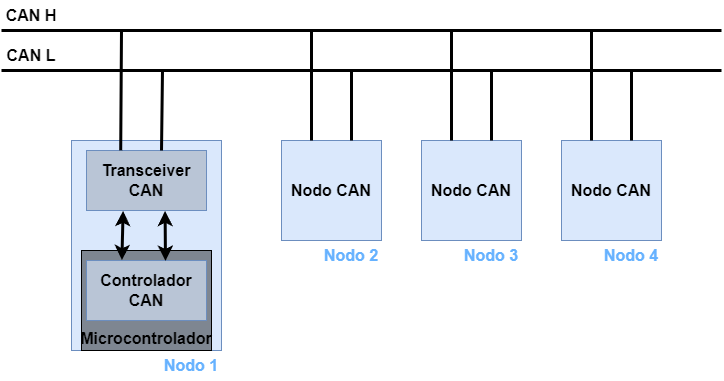
\includegraphics[scale=.5]{./Figures/CANBUS_Esquema.png}
	\caption{Esquema de red CAN.}
	\label{fig:canBus}
\end{figure}

%----------------------------------------------------------------------------------------

\section{Servomotores}

Un servomotor \citep{Industrial_Automation_Hands_On} es un tipo de motor eléctrico que tiene la capacidad de controlar la posición angular de su eje, así como la velocidad de rotación y el torque de salida. Esto se consigue con la utilización de un sistema de lazo cerrado de control que se retroalimenta con un sensor de posición angular llamado \textit{encoder}. En general, el tipo de bobinas del motor eléctrico no determina la condición de servomotor, sino que este cuente con las cualidades de control descriptas. En la figura \ref{fig:servomotor} \citep{web_partes_servomotor} se pueden observar las distintas partes que conforman un servomotor.

\begin{figure}[htbp]
	\centering
	\includegraphics[scale=0.8]{./Figures/servomotor.jpg}
	\caption{Partes de un servomotor\protect\footnotemark .}
	\label{fig:servomotor}
\end{figure}

\footnotetext{\url{https://www.logicbus.com.mx/blog/wp-content/uploads/2021/03/que-es-un-servomotor-773x400.jpg}} %Link a imagen de servomotor

%----------------------------------------------------------------------------------------

\section{Proyecto SN-17}

El proyecto SN-17 (Servo NEMA 17) es un sistema desarrollado como emprendimiento personal (A3 Engineering) que adapta motores eléctricos del tipo paso a paso o \textit{steppers} para funcionar como servomotores. El sistema SN-17 agrega un \textit{encoder} y un \textit{driver} al motor, los cuales generan un lazo cerrado, logrando así que el motor tenga las funcionalidades de un servomotor. En la figura \ref{fig:SN17} se puede observar una placa de control SN-17. Esta se coloca en la parte trasera del motor paso a paso.

\begin{figure}[htbp]
	\centering
	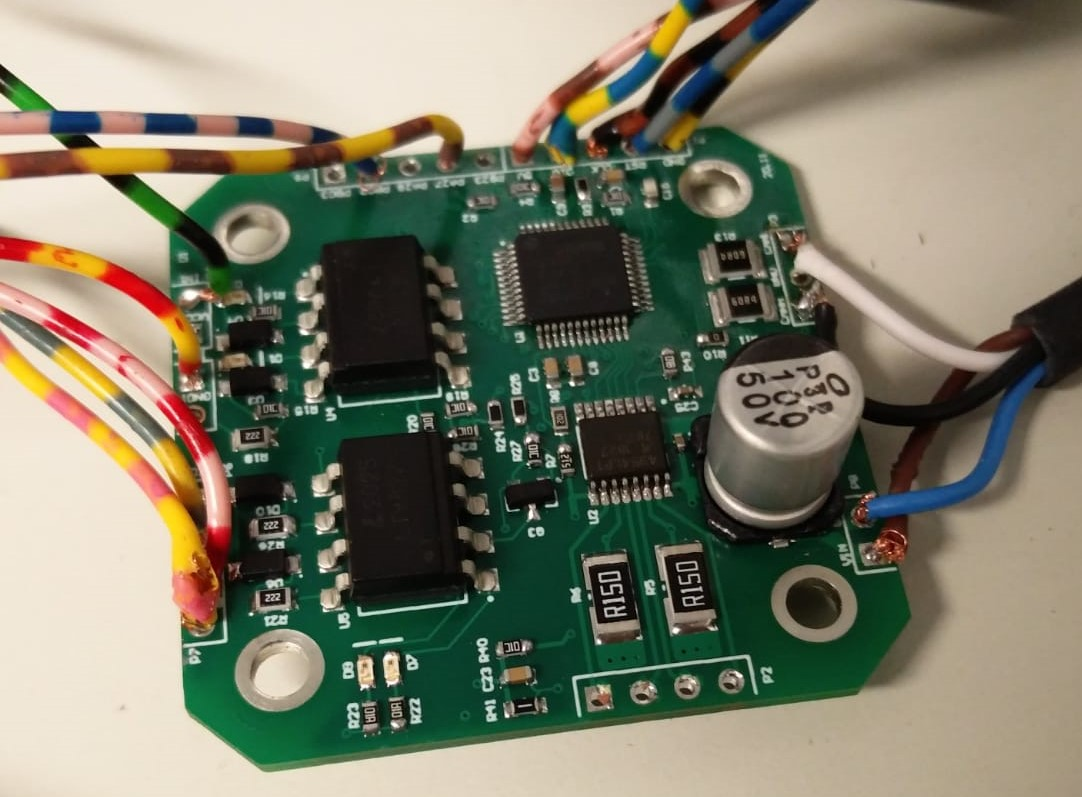
\includegraphics[scale=.3]{./Figures/SN17_5.jpeg}
	\caption{Plaqueta SN-17.}
	\label{fig:SN17}
\end{figure}

Además de generar las funcionalidades mencionadas, el sistema SN-17 utiliza señales discretas industriales que le permiten comunicarse con controladores de uso industrial (\textit{Programmable Logic Controllers} o PLCs).

Actualmente se está trabajando en implementar estos sistemas en la planta de la empresa Cambre ICyFSA \citep{web_cambre}, donde se están construyendo distintos dispositivos para aplicaciones industriales con estos motores. En la figura \ref{fig:aplicacionSN17} se puede observar un dibujo CAD de un actuador lineal con un sistema SN-17 implementado. Este funciona como un prensador en un proceso industrial.

\begin{figure}[h!]
	\centering
	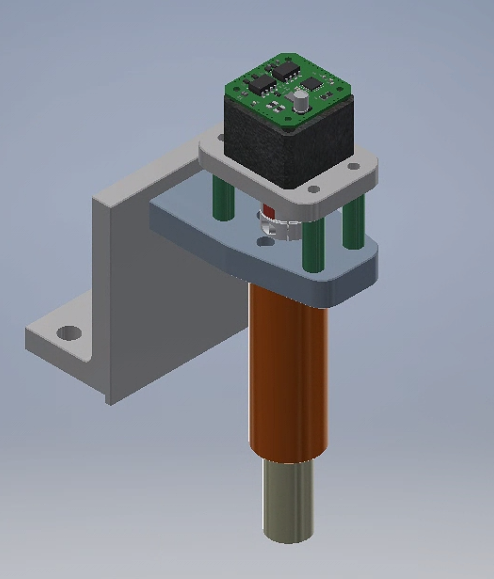
\includegraphics[width=0.7\linewidth ,height=0.3\textheight]{./Figures/Prensador-N17.PNG}
	\caption{Actuador lineal con SN-17.}
	\label{fig:aplicacionSN17}
\end{figure}

%----------------------------------------------------------------------------------------

\section{Motivación}
\label{motivacion}

En la actualidad el ámbito de actuadores industriales está principalmente dominado por aquellos de carácter neumático \citep{web_actuator_market}. Sin embargo, en los últimos años el uso de actuadores eléctricos ha empezado a ser más significativo debido a las mayores aptitudes de control que poseen y a sus menores costos operativos \citep{web_comparacion_actuadores}. En la tabla \ref{tab:comparacion_neumatico_electrico} se muestra una comparativa de ambos tipos de actuadores.

\begin{table}[htpb]
	\centering
	\caption[Comparación de actuadores neumáticos y eléctricos]{Comparación de actuadores neumáticos y eléctricos.}
	\begin{tabular}{c  c  c}    
		\toprule
		 	 & \textbf{Actuadores neumáticos}  & \textbf{Actuadores eléctricos}\\
		\midrule
		\textbf{Diseño} 			& Simple 		& Complejo  \\
		\textbf{Implementación} 	& Simple 		& Complejo \\			
		\textbf{Fuerza} 			& Según presión de aire	& Según reducción mecánica \\
		\textbf{Presición}			& Baja 	& Alta \\
		\textbf{Repetitibilidad}	& Baja 	& Alta \\
		\textbf{Eficiencia}			& Baja 	& Alta \\
		\textbf{Control de movimiento}	& Bajo 	& Alto \\
		\textbf{Mantenimiento}	& Alto 	& Bajo \\
		\bottomrule
		\hline
	\end{tabular}
	\label{tab:comparacion_neumatico_electrico}
\end{table}

Los actuadores eléctricos suelen emplear un servomotor en su interior que, junto con un mecanismo, generan el movimiento deseado con una precisión superior a los actuadores neumáticos. Aún así, este tipo de actuadores tienen como problema su elevado costo de adquisición y su dificultad de implementación, que limitan su uso. En este contexto, la organización A3 Engineering desarrolló el sistema SN-17 en un intento de disminuir los costos de los servomotores de aplicaciones pequeñas y, en un futuro, de los actuadores eléctricos.

La empresa Cambre ICyFSA instaló una serie de sistemas SN-17 en su planta productiva con resultados iniciales exitosos. Sin embargo, se limitó la implementación de más sistemas debido a su dificultad para reprogramarlos en momentos de necesidad. Esto se debe a que requieren de un cambio de \textit{firmware} para modificar su configuración y esto solo puede ser realizado por personal calificado. La motivación de este trabajo es brindar una interfaz para programación y monitoreo de una red de motores que pueda ser utilizada por personal no especializado.


%----------------------------------------------------------------------------------------

\section{Estado del arte}
\label{estado_del_arte}

Actualmente existe una extensa oferta de servomotores y motores paso a paso en el mercado. En general, lo que en el ámbito industrial se refiere a servomotores \citep{Industrial_Automation_Hands_On} son motores del tipo DC \textit{brushless} o AC de inducción (monofásicos y trifásicos). Estos tienen un precio significativamente mayor que los \textit{steppers} y suelen requerir de \textit{drivers} externos y, en caso de motores AC, variadores de frecuencia. En los casos en que se requiere alta potencia o alto rendimiento, estos servos son la opción indicada. Requieren de técnicos capacitados para su programación y ofrecen interfaces de usuario avanzadas. En general, representan soluciones de alto costo. Un motor AC de la empresa Panasonic \citep{web_servo_panasonic} junto con su \textit{driver} se presenta en la figura \ref{fig:ac-servo}. 


\begin{figure}[h!]
	\centering
	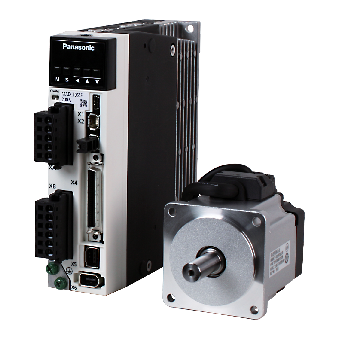
\includegraphics[scale=.65]{./Figures/ac-servo.png}
	\caption{Servomotor AC con \textit{driver}\protect\footnotemark.}
	\label{fig:ac-servo}
\end{figure}

\footnotetext{\url{https://assets.content.na.industrial.panasonic.com/public/styles/large/public/2019-11/A6_Servo_\%26_Drive_PHOTO_RGB_Panasonic_11-01-19.png?VersionId=Zy2t46MH7Tk5ce_Pw18lIwmTNWsf4YoK&itok=hJTUelmJ}} 


Por otro lado, en lo referido a motores \textit{steppers}, la oferta también es variada. Estos pueden adquirirse a precios muy accesibles y en distintos tamaños con lazo de control abierto. Requieren el uso de un \textit{driver} externo para su operación y su programación suele hacerse con software de terceros. Según la aplicación pueden requerir de conocimientos técnicos elevados. También existen variantes que agregan un \textit{encoder} de posición angular,  llamados \textit{closed loop steppers}. Estos solventan uno de los mayores problemas de estos motores relacionado con la pérdida de posición en caso de una perturbación, pero no permiten entregar torque constante. También requieren de \textit{drivers} externos y, según el fabricante, las interfaces de programación pueden ser complejas. Un ejemplo de un \textit{closed loop stepper} \citep{web_closed_loop_stepper} se presenta en la figura \ref{fig:closed-loop-stepper}, junto con su \textit{driver} correspondiente.

\begin{figure}[h!]
	\centering
	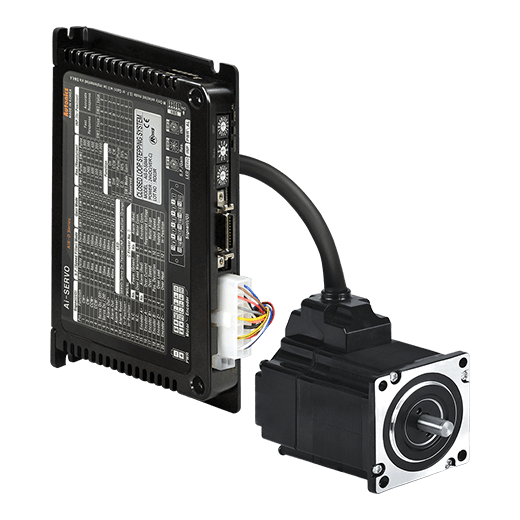
\includegraphics[scale=.35]{./Figures/closed_loop_stepper.png}
	\caption{\textit{Closed loop stepper} con \textit{driver}\protect\footnotemark .}
	\label{fig:closed-loop-stepper}
\end{figure}

\footnotetext{\url{https://www.autonics.com/web/2022/12/29/6/46/15/1032047e-1a41-4c24-aee4-966f2109fd40.png}} %Link a imagen de closed loop stepper

Finalmente, existen placas de control que, además de funcionar como un \textit{closed loop stepper}, tienen un \textit{driver} incorporado que permite controlar los motores de forma diferente, logrando entregar torque constante. El problema principal de estas soluciones es que suelen tener características de \textit{hobbista} y no son aptas para ámbitos industriales. También requieren de elevado conocimiento técnico para su programación debido a la falta de interfaces de usuario. En la figura \ref{fig:mechaduino} se puede ver un ejemplo de una de estas placas llamada \textit{Mechaduino} \citep{web_mechaduino}.

\begin{figure}[h!]
	\centering
	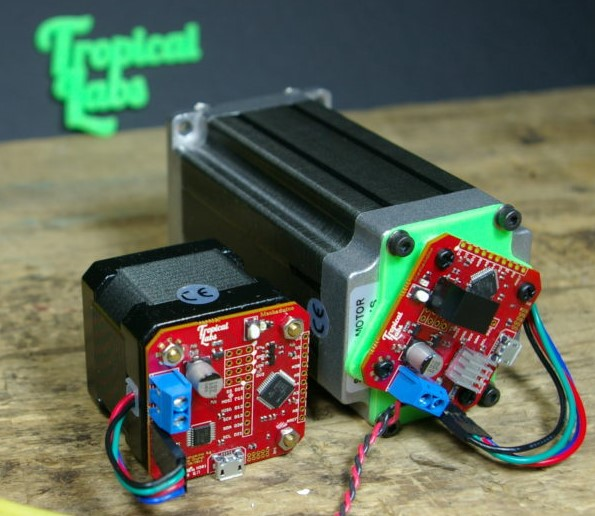
\includegraphics[scale=.6]{./Figures/mechaduino.jpg}
	\caption{Proyecto Mechaduino\protect\footnotemark .}
	\label{fig:mechaduino}
\end{figure}

\footnotetext{\url{https://tropical-labs.com/wp-content/uploads/2018/10/IMGP1300-1-1024x681.jpg}} %Link a imagen de mechaduino

En la Tabla \ref{tab:servos} se resume la información de los distintos tipos de motores mencionados.


\begin{table}[h!]
	\centering
	\caption[Estado del arte]{Resumen de características de servomotores.}
	\begin{tabular}{c c c c c}    
		\toprule
		\textbf{Motor} 	 & \textbf{Lazo de control}  & \textbf{\textit{Driver}} & \textbf{Programación} & \textbf{Precio (USD)} \\
		\midrule
		Servomotor & Cerrado & Externo & Compleja 	& >  1.500 \\		
		\textit{Stepper open loop} & Abierto & Externo & Intermedia 	&  300\\
		\textit{Stepper closed loop} & Cerrado s/torque	& Externo & Intermedia 	&  400\\
		\textit{Mechaduino} & Cerrado	& Interno & Compleja 	&  200 \\
		SN-17 + interfaz	& Cerrado	& Interno & Simple 		&  300 \\
		\bottomrule
		\hline
	\end{tabular}
	\label{tab:servos}
\end{table}
%----------------------------------------------------------------------------------------

\section{Objetivos y alcance}

El objetivo de este trabajo es proporcionar una interfaz de usuario para el sistema SN-17 que permita que un operario no especializado pueda modificar los programas de los distintos motores conectados a través de una red CAN. La interfaz también debe poder emplearse para monitorear el estado de los motores conectados cuando están operativos. 

El proyecto incluye:

\begin{itemize}
	\item Una interfaz de usuario que permita configurar y supervisar los servomotores conectados.
	\item La construcción e implementación de la estructura de mensajes CAN.
	\item La configuración de la red CAN.
	\item El desarrollo y fabricación de una plaqueta con el sistema embebido.
	\item El desarrollo del firmware para este sistema y la adaptación del firmware del sistema SN-17.
\end{itemize}



\chapter{Introducción específica} % Main chapter title

\label{Chapter2}

%----------------------------------------------------------------------------------------
%	SECTION 1
%----------------------------------------------------------------------------------------
Este capítulo aborda una explicación más detallada de algunos de los puntos explicados en el capítulo anterior, como el sistema SN-17 y el protocolo CAN. También, se presentan algunas características de las entradas y salidas de los controladores industriales PLCs y se explican los distintos componentes seleccionados para el trabajo y su funcionamiento.

\section{Especificaciones SN-17}

El sistema SN-17 se desarrolló para controlar motores \textit{stepper} pequeños del tipo NEMA 17. Este es un estándar ampliamente utilizado para este tipo de motores, que indica las dimensiones que deben tener. Mediante una adaptación mecánica, también se puede emplear la plaqueta para controlar motores de menor o mayor tamaño, siempre y cuando sean del tipo \textit{stepper} y no requieran corrientes mayores a 2 A.

El sistema se alimenta comúnmente con 24 V, con lo que se alimentan las bobinas del motor y el regulador de tensión de 5 V con el cuál se alimenta la electrónica de la plaqueta. Esto está compuesto por un encoder magnético \citep{web_AS5047D}, que permite sensar la posición angular del eje del motor; un \textit{driver} del tipo doble puente H\citep{web_A4954}, que controla la corriente que circula por las bobinas del motor; un \textit{transciever} CAN\citep{web_transciever_CAN}, que convierte y recibe las señales eléctricas del bus CAN; y un microcontrolador ATMSAMC21\citep{web_ATSAMC21G18A}, encargado de controlar el proceso. En lo que respecta al microcontrolador, este cuenta con una arquitectura M0+ y tiene, entre sus periféricos, un controlador CAN incorporado.

La plaqueta cuenta con un circuito de entradas y salidas del tipo PNP que se encuentran eléctricamente aisladas del microcontrolador usando optoacopladores\citep{web_optoacopladores_LTV}. Estas pueden alimentarse a tensiones distintas que el resto del sistema y se usan para interactuar con un controlador industrial del tipo PLC.

El sistema tiene un ciclo de control de lazo cerrado del tipo PID\citep{paper_PID_steppers} al cual se le indica un valor deseado (\textit{set point}) de posición, velocidad o torque. Con esta información, se la compara con los valores obtenidos del encoder y se determina cómo deben ser alimentadas las bobinas del motor para alcanzar el \textit{set point}. Para el funcionamiento de esto, el encoder debe ser calibrado junto con el motor, mediante una rutina en la que se arma una tabla de referencia que luego es usada en operación.

Sobre el control mencionado, corre una aplicación en la que se cargan programas que el motor debe realizar. Estos programas estan compuestos de instrucciones configurables, que permiten establecer los modos de control deseados (posición, velocidad o torque), los \textit{set points} y errores admisibles para estos (\textit{thresholds}), una limitación del torque para esa instrucción, los tiempos que deben cumplirse para considerar correcta la instrucción (\textit{hold time}) y los tiempos para que se considere que el sistema entró en estado de error (\textit{timeout}). Otras instrucciones tienen que ver con flujo de programa, interacción con las entradas y salidas y comunicaciones a través del puerto CAN.

Existen también configuraciones que se le pueden aplicar al motor, estas son:
\begin{itemize}
	\item Constantes PID del lazo de control
	\item Tipo de rutina de \textit{homing} del motor
	\item Funcionamiento de entradas y salidas
	\item Guardado de posiciones de eje en memoria
\end{itemize}

El sistema también puede recibir comandos de forma manual:
\begin{itemize}
	\item Calibración de encoder y motor
	\item Activación o apagado de motor
	\item Cerado de motor
	\item Activación de salidas
\end{itemize}

En la Tabla \ref{tab:sn17_hoy} se resume la información sobre las distintas funciones que la aplicación del sistema SN-17 puede realizar.

\begin{table}[h]
	\centering
	\caption[Operaciones SN-17]{Funciones de SN-17}
	\begin{tabular}{c c c}    
		\toprule
		\textbf{Señal} 	 & \textbf{Tipo}  & \textbf{Descripción}\\
		\midrule
		Tipo de instrucción & Instrucción 	& Define la instrucción\\		
		Límite de torque 	& Instrucción	& Torque máximo de instrucción \\
		Modo de control		& Instrucción 	& Posición, velocidad, torque \\
		\textit{Set point}	& Instrucción 	& Valor de lazo de control \\
		\textit{Threshold}	& Instrucción 	& Valor de error admisible \\
		\textit{Hold time}	& Instrucción 	& Tiempo de cumplimiento \\
		\textit{Timeout}	& Instrucción 	& Tiempo de no cumplimiento \\
		Guardar posición	& Configuración & Guarda posición actual \\
		Constantes PID		& Configuración & Constantes lazo de control \\	
		Entradas y salidas	& Configuración & Funcionamiento de las IO \\
		\textit{Homing}		& Configuración & Establece rutina de cerado \\	
		Calibración			& Comando		& Inicia la rutina de calibración \\
		Activar motor		& Comando		& Enciende/apaga el motor \\
		\textit{Go Home}	& Comando		& Inicia la rutina de cerado \\
		Activar salidas		& Comando		& Enciende/apaga salidas \\	
		\bottomrule
		\hline
	\end{tabular}
	\label{tab:sn17_hoy}
\end{table}

\section{Características del protocolo CAN}

Como se trató en el capítulo 1, el protocolo CAN está estandarizado en la norma internacional ISO 11898\citep{web_ISO_CAN}. El estándar abarca solamente las capas física y de enlace de datos, es decir, las 2 capas más bajas en un modelo OSI - \textit{Open System Interconection}, como el que se puede ver en la Figura \ref{fig:modeloOsi}. Para las capas superiores, existen otros estándares, como CANOpen\protect\footnotemark, del cual se tomaron ideas para este trabajo, pero no se implementa en si.

\begin{figure}[htbp]
	\centering
	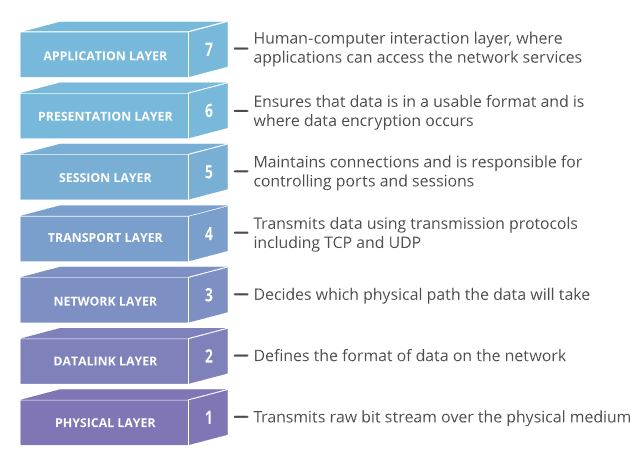
\includegraphics[scale=.8]{./Figures/OSI_model.JPG}
	\caption{Modelo de capas OSI\protect\footnotemark}
	\label{fig:modeloOsi}
\end{figure}

\footnotetext{\url{https://www.can-cia.org/canopen/}} %Link a CANOpen

\footnotetext{\url{https://www.cloudflare.com/es-es/learning/ddos/glossary/open-systems-interconnection-model-osi/}} %Link a imagen de modelo OSI

Otras características que tiene la red están relacionadas con el armado del circuito de los nodos, el cual suele estar especificado en las hojas de datos de los \textit{transcievers}, así como la necesidad de colocar una resistencia de terminación en los extremos de la red, como puede visualizarse en la Figura \ref{red_can_con_resistores}. El valor de esta resistencia depende de muchas variables, como el largo de la red y la velocidad de transmisión y suelen usarse guías para seleccionarlas. Los medios físicos de transmisión, así como los conectores no estás especificados por la norma, aunque existen recomendaciones \citep{Embedded_Networking_CAN}.

\begin{figure}[htbp]
	\centering
	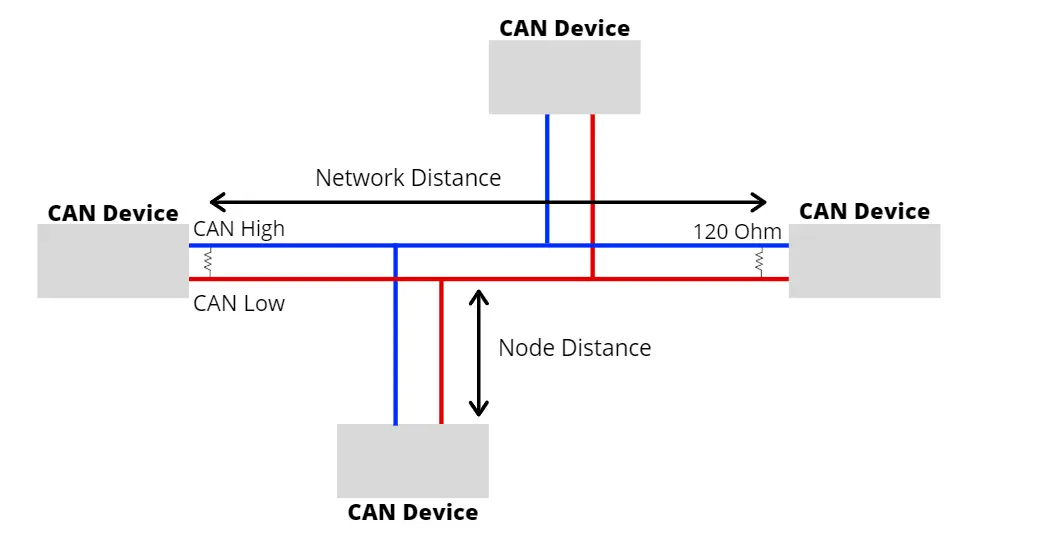
\includegraphics[scale=.6]{./Figures/canBus.png}
	\caption{Esquema de red CAN con resistores de terminación\protect\footnotemark}
	\label{fig:red_can_con_resistores}
\end{figure}

\footnotetext{\url{https://www.seeedstudio.com/blog/2019/11/27/introduction-to-can-bus-and-how-to-use-it-with-arduino/}} %Link a imagen de Red CAN

Las señales usadas son del tipo diferencial y se clasifican en dominantes y recesivas. Una señal dominante en el bus tiene prioridad por sobre una señal recesiva, lo que permite que varios dispositivos estén conectados y puedan hablar al mismo tiempo y que se puedan detectar colisiones\citep{Embedded_Networking_CAN}. En un estado recesivo, las líneas CAN-H y CAN-L están al mismo nivel de tensión, generalmente 2.5 V en sistemas embebidos, aunque el estándar indica otros valores adicionales de tensión admitidos. En un estado dominante, CAN-L baja, al menos 1 V, mientras que CAN-H sube, al menos, 1 V generando una diferencia entre ambos. 

El bus CAN se caracteriza por ser asincrónico, es decir, no tener una línea de reloj. Para sincronización, se usa un método conocido como \textit{Non Return To Zero} o NRZ. Este consiste en determinar una cantidad máxima de bits que pueden ser transmitidos en el bus sin una transición entre estados recesivos y dominantes. En cada transición, los nodos se resincronizan, evitando largas cadenas de mensajes no coordinadas. Entonces, para lograr esto, CAN emplea el \textit{Bit-Stuffing} que fuerza el cambio de estado en la línea cada 5 bits iguales. 

El estándar también subdivide el tiempo de un bit en distintos segmentos: Sincronización, propagación, fase 1 y fase 2. Estos se describen en una unidad de tiempo menor, referida como \textit{time quanta}. Para un buen funcionamiento de la red, todos estos parámetros deben ser correctamente configurados en los distintos nodos CAN.

En lo que respecta a las tramas CAN, existen de 2 tipos: estándar y extendida. En este trabajo el enfoque está en las tramas estándar que se caracterizan por tener un identificador de 11 bits, donde se encodea información del receptor del mensaje. En la Figura \ref{fig:trama_can} se puede ver un esquema detallando la trama CAN estándar. La trama se separa en:
\begin{itemize}
	\item Comienzo de trama - \textbf{SOF}
	\item Arbitraje
	\item Control
	\item Data a envíar
	\item Verificación
	\item Reconocimiento - \textit{Acknowledge}
	\item Fin de trama - \textbf{EOF}
\end{itemize} 

\begin{figure}[htbp]
	\centering
	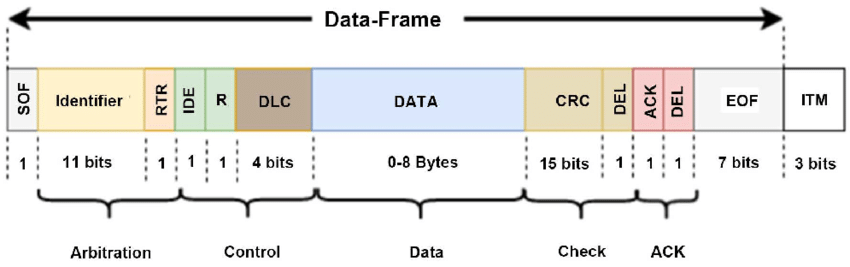
\includegraphics[scale=.5]{./Figures/CANBUS-frame.png}
	\caption{Trama CAN estándar\protect\footnotemark}
	\label{fig:trama_can}
\end{figure}

\footnotetext{\url{https://www.researchgate.net/publication/328607559_Classification_Approach_for_Intrusion_Detection_in_Vehicle_Systems}} %Link a imagen de trama CAN

La sección de arbitrake está compuesto por el identificador y el bit RTR (\textit{Remote Transmission Request}), que se utiliza para pedir a la red que se transmita cierto mensaje. El identificador es procesado por cada nodo de la red y, mediante el uso conjunto de máscaras y filtros, determinan si el mensaje corresponde al nodo o no. También, en caso de que 2 o más nodos quieran transmitir un mensaje al mismo tiempo, el que lo haga con el identificador más bajo será el que tendrá prioridad y tomará el control de la red. Esta funcionalidad se consigue gracias a la lógica AND del circuito del bus. Los nodos que no logran transmitir su mensaje, debido a la prioridad inferior, pueden identificar esto y retransmitir cuando el bus esté nuevamente desocupado. 

El campo de control del frame tiene al bit IDE, que identifica el tipo de trama entre estándar y extendida y el DLC, donde se indica la cantidad de bytes que tendrá el mensaje. Esta puede ser entre 0 y 8 bytes de largo.

Luego de el envío de la data, se encuentran los campos de verificación y reconocimiento. La verificación está compuesta por el campo CRC, que permite comprobar que la información transmitida es igual a la información recibida, es decir, que no haya habido errores de transmisión. Luego de esto, viene el sector de reconocimiento, donde lo receptores reconocen que el mensaje se ha recibido correctamente enviando un bit dominante. La trama termina con una sección de fin de trama.

En la actualidad, se comercializan una gran cantidad de controladores CAN. La gran mayoría ofrece todas las funcionalidades descriptas, que son lo requerido por el estándar. Según la aplicación, se pueden elegir controladores que tengan distinto número de filtros y máscaras para identificación de mensajes, tamaño de buffer de mensajes, tanto de recepción como de transmisión, velocidad de operación, entre muchas otras. También, muchos microcontroladores incluyen un periférico de CAN, que suele ser una solución conveniente para implementar redes de este tipo. Una vez elegido el controlador, la hoja de datos indica cómo deben configurarse los distintos parámetros. Esto, como se explicó, debe hacerse de forma correcta para asegurar un buen funcionamiento de la red.

\section{Entradas y salidas de controladores industriales}

Un PLC - \textit{Programmable Logic Controller} es un tipo de controlador ampliamente utilizado para manejar procesos industriales. Se caracterizan por su robustez y su forma de programación, muy similar a la lógica de relé.

En general, los PLC requieren interactuar con gran número de sensores y actuadores presentes en un proceso, por lo que cuentan con amplios módulos de entradas y salidas digitales. Estos módulos suelen adaptar el nível de tensión de las señales que reciben y transmiten y suelen proteger los circuitos internos del PLC aislando eléctricamente las señales\citep{Introduction_Industrial_Automation}. Normalmente, el estándar industrial es trabajar a 24 V de corriente contínua, aunque también es común usar 48 V DC o corrientes AC de línea y, en casos poco frecuentes, pueden aparecer otros valores. Los controladores industriales suelen estar preparados para trabajar con la mayoría de estas condiciones.

Uno de los circuitos de acondicionamiento de salidas de PLC se puede observar en la Figura \ref{fig:Circuito_NPN}. En este caso es del tipo NPN, que hace referencia al transistor empleado y el tipo de conexión externa que requiere para su línea común. Notar el uso de un opto acoplador para separar eléctricamente los circuitos y la cantidad de elementos de protección que se agregan para dar robustez. Existen también circuitos del tipo PNP, que cambian el transistor que emplean y el conexionado, y también hay con relés.

\begin{figure}[htbp]
	\centering
	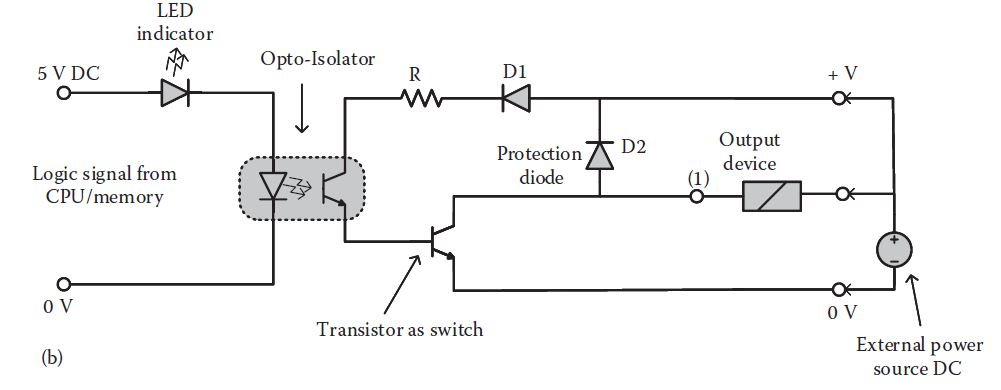
\includegraphics[scale=.6]{./Figures/Circuito_NPN.JPG}
	\caption{Circuito NPN\citep{Introduction_Industrial_Automation}}
	\label{fig:Circuito_NPN}
\end{figure}

Para especificar un módulo de entradas o de salidas, normalmente se deben especificar los rangos de voltaje y corriente de operación, el consumo máximo de corriente, los valores de tensión lógicos y la velocidad y frecuencia de conmutación.

En el mercado existen gran variedad de controladores industriales, cada uno con distintos módulos de entradas y salidas y distintos periféricos disponibles, según la aplicación. 

\section{Características de componentes electrónicos empleados}

En esta sección se dará una explicación de los distintos componentes electrónicos usados en este trabajo. Se tratará sobre su funcionamiento y sobre los recursos disponibles para trabajar con ellos.

\subsection{Pantallas LED y conversores I2C}

Las pantallas LCD ofrecen una forma conveniente y económica para generar una interfaz de usuario. Para los proyectos de electrónica, uno de los modelos más populares es el panel de texto basado en el Hitachi HD44780\citep{Arduino_Cookbook}. En la Figura \ref{Pantalla_LCD} se muestra uno de estos displays, en particular uno de 4 líneas y 20 caracteres por línea. Estos dispositivos solo pueden representar caracteres, no pueden hacer dibujos ni gráficos, por lo tanto las interfaces que se obtienen son sencillas.

\begin{figure}[htbp]
	\centering
	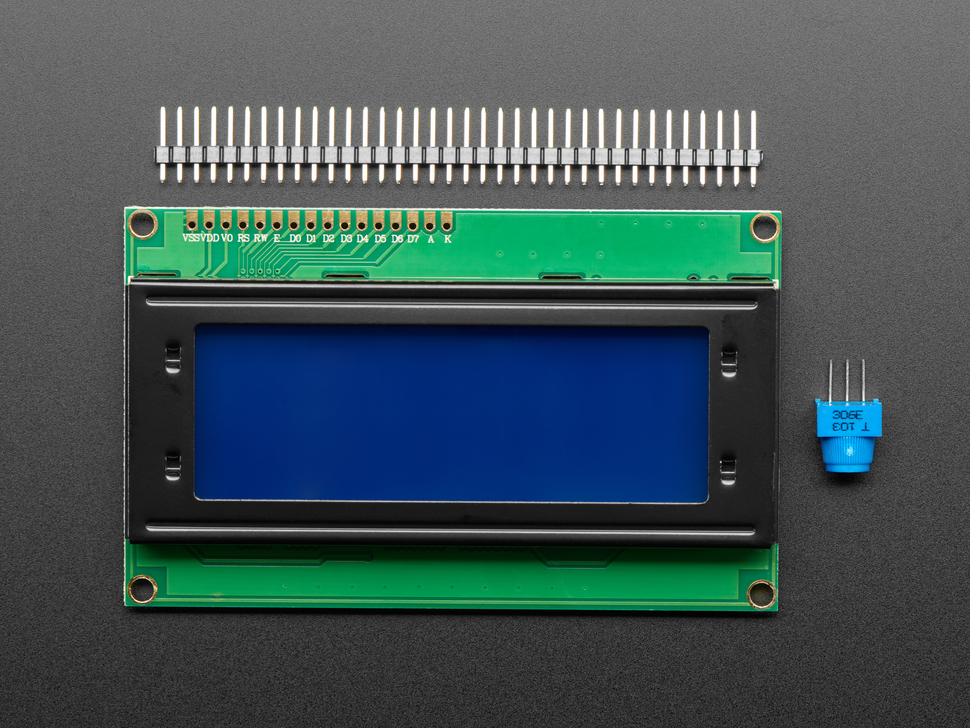
\includegraphics[scale=1]{./Figures/LCD.jpg}
	\caption{Pantalla LCD 20x4\protect\footnotemark}
	\label{fig:Pantalla_LCD}
\end{figure}

\footnotetext{\url{https://www.adafruit.com/product/198}} %Link a imagen de LCD

Existen modelos de LCD que incluyen una interfaz I2C (\textit{Inter-Integrated Circuit}), un protocolo de comunicación simple, muy utilizado en sistemas embebidos. Esta interfaz facilita la interacción con el display, que normalmente requiere una serie de conexiones discretas para controlarlo. De esta manera, se pueden envíar comandos para modificar la configuración del dispositivo o mostrar texto, según se requiera.

La mayoría de microcontroladores que se emplean en la actualidad tienen un periférico de I2C e incluyen drivers de este, lo que también promueve la implementación de las interfaces. El protocolo es del tipo serial y sincrónico, requiriendo 2 líneas de información, SDA y SCL, por donde se transmite la data y el reloj, respectivamente. En un bus I2C, los distintos dispositivos conectados tienen un código identificador que se emplea para controlar las comunicaciones.

A la hora de implementar una solución con este tipo de pantallas, puede tomarse de referencia alguna de las librerías de código abierto que se encuentran disponibles en la web. Esto puede ayudar a reducir significativamente los tiempos de desarrollo y es el camino que se tomó en este trabajo.

\subsection{Matriz de botones}

Las matrices de botones consisten en un conjunto de contactos normalmente abiertos que conectan una fila con una columna cuando se presionan. La metodología de uso consiste en conectar las filas a pines de entrada con resistores de pull-up en el microcontrolador y las columnas a pines de salida. La secuencia que se realiza es poner el nivel de tensión de una columna por vez en bajo (mientras las otras se mantienen en un nivel alto). En ese momento, se leen las entradas de las filas, si alguna está en un nivel bajo es indicación de que el botón de esa fila y columna fue presionado (ya que normalmente estarían en un nivel alto por las resistencias de pull-up)\citep{Arduino_Cookbook}. En la Figura \ref{fig:but_matrix} se puede visualizar un esquema de conexionado de una matriz de botones 3x3 a un microcontrolador. Notar también que se muestran los conexionados internos de la matriz, de las filas y las columnas.

\begin{figure}[htbp]
	\centering
	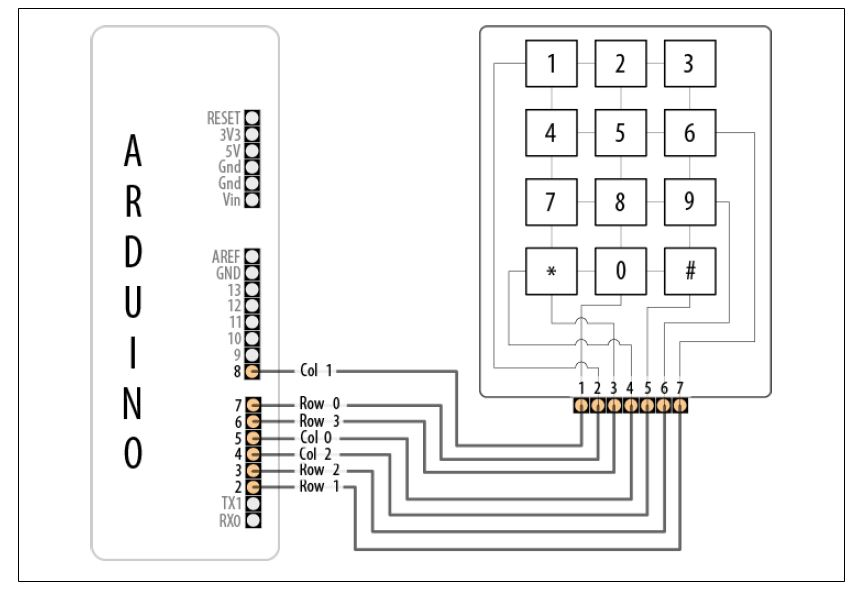
\includegraphics[scale=.6]{./Figures/But_Matrix.JPG}
	\caption{Conexión de matriz de botones 3x3\citep{Arduino_Cookbook}}
	\label{fig:but_matrix}
\end{figure}

Como en el caso de las pantallas LCD, existen muchas librerías de código abierto que implementan soluciones de matrices de botones. Se considera conveniente consultarlas si se desea utilizar uno de estos dispositivos, y es lo que se hizo en este trabajo.

\subsection{Conversores UART-USB}

El \textit{Universal Asynchronous Receive Transmit} o UART, es un protocolo serial de comunicación ampliamente utilizado en sistemas embebidos. Se caracteriza, principalmente, por su sencillez. Como su nombre indica, es un protocolo asincrónico (sin línea de clock), que requiere solamente 1 línea para envíar data, o 2 para envíar y recibir.

La gran mayoría de los microcontroladores que se utilizan actualmente cuentan con un periférico de UART y se suelen incluír drivers de este. Esto reduce los tiempos a la hora de desarrollar una implementación.

Otro protocolo ampliamente usado es el USB, y suele ser el preferido para interactuar con una PC. Existen en el mercado una gran cantidad de conversores que transforman un mensaje UART a uno USB, permitiendo la interacción entre una PC y un sistema embebido. En general, estos conversores cuentan con drivers para los distintos sistemas operativos y son reconocidos por estos, por lo cual solo es necesario conectarlos a través del puerto USB. Desde la PC, cualquier programa de monitoreo de puertos seriales puede usarse para envíar y recibir mensajes con el sistema embebido.

Este tipo de implementaciones suele ser muy útil para realizar operaciones de búsqueda de errores o para armar interfaces gráficas con una PC, facilitando la operatoria de un usuario final. En este trabajo se utiliza uno de estos módulos para esta finalidad.

\chapter{Diseño e implementación} % Main chapter title

Este capítulo presenta la arquitectura del sistema embebido, la estructura de los componentes de software principales, las consideraciones en la selección de componentes electrónicos, el diseño del PCB y el gabinete del sistema.

\label{Chapter3} % Change X to a consecutive number; for referencing this chapter elsewhere, use \ref{ChapterX}

\definecolor{mygreen}{rgb}{0,0.6,0}
\definecolor{mygray}{rgb}{0.5,0.5,0.5}
\definecolor{mymauve}{rgb}{0.58,0,0.82}

%%%%%%%%%%%%%%%%%%%%%%%%%%%%%%%%%%%%%%%%%%%%%%%%%%%%%%%%%%%%%%%%%%%%%%%%%%%%%
% parámetros para configurar el formato del código en los entornos lstlisting
%%%%%%%%%%%%%%%%%%%%%%%%%%%%%%%%%%%%%%%%%%%%%%%%%%%%%%%%%%%%%%%%%%%%%%%%%%%%%
\lstset{ %
  backgroundcolor=\color{white},   % choose the background color; you must add \usepackage{color} or \usepackage{xcolor}
  basicstyle=\footnotesize,        % the size of the fonts that are used for the code
  breakatwhitespace=false,         % sets if automatic breaks should only happen at whitespace
  breaklines=true,                 % sets automatic line breaking
  captionpos=b,                    % sets the caption-position to bottom
  commentstyle=\color{mygreen},    % comment style
  deletekeywords={...},            % if you want to delete keywords from the given language
  %escapeinside={\%*}{*)},          % if you want to add LaTeX within your code
  %extendedchars=true,              % lets you use non-ASCII characters; for 8-bits encodings only, does not work with UTF-8
  %frame=single,	                % adds a frame around the code
  keepspaces=true,                 % keeps spaces in text, useful for keeping indentation of code (possibly needs columns=flexible)
  keywordstyle=\color{blue},       % keyword style
  language=[ANSI]C,                % the language of the code
  %otherkeywords={*,...},           % if you want to add more keywords to the set
  numbers=left,                    % where to put the line-numbers; possible values are (none, left, right)
  numbersep=5pt,                   % how far the line-numbers are from the code
  numberstyle=\tiny\color{mygray}, % the style that is used for the line-numbers
  rulecolor=\color{black},         % if not set, the frame-color may be changed on line-breaks within not-black text (e.g. comments (green here))
  showspaces=false,                % show spaces everywhere adding particular underscores; it overrides 'showstringspaces'
  showstringspaces=false,          % underline spaces within strings only
  showtabs=false,                  % show tabs within strings adding particular underscores
  stepnumber=1,                    % the step between two line-numbers. If it's 1, each line will be numbered
  stringstyle=\color{mymauve},     % string literal style
  tabsize=2,	                   % sets default tabsize to 2 spaces
  title=\lstname,                  % show the filename of files included with \lstinputlisting; also try caption instead of title
  morecomment=[s]{/*}{*/}
}


%----------------------------------------------------------------------------------------
%	SECTION 1
%----------------------------------------------------------------------------------------
\section{Arquitectura del sistema embebido}

En la figura \ref{fig:arquitectura_sistema} se muestra un diagrama de bloques con la arquitectura del sistema SCI-CAN y sus interacciones. El recuadro marcado como controlador corresponde a lo desarrollado en este trabajo. En los recuadros externos están los dispositivos con los que este sistema debe interactuar: PLCs, servomotores SN-17 y PC.

La interacción con los PLC es a través de señales discretas que necesitan estar acondicionadas según especificaciones \citep{plan_trabajo}. Con los servomotores la comunicación es a través de un bus CAN y la interacción con una PC se consigue utilizando un conversor USB - UART.

\begin{figure}[htbp]
	\centering
	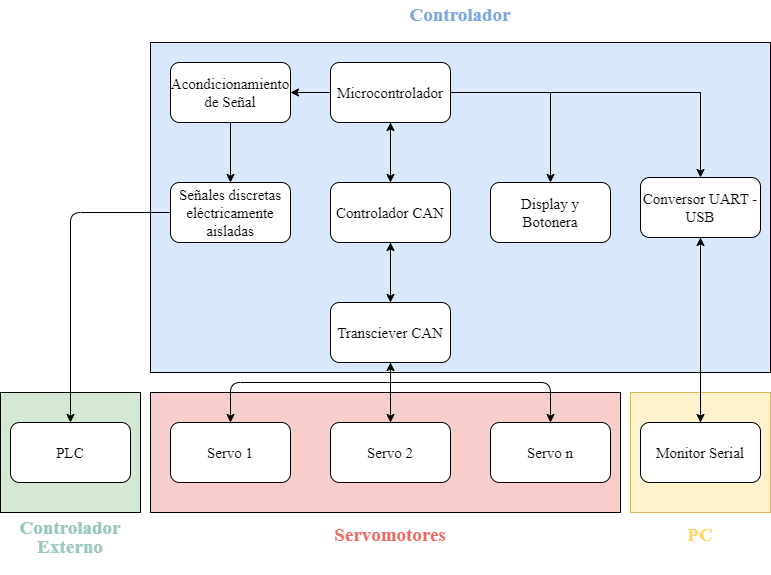
\includegraphics[scale=.5]{./Figures/Arquitectura_SE.png}
	\caption{Arquitectura del sistema.}
	\label{fig:arquitectura_sistema}
\end{figure}

Las interacciones internas del sistema incluyen:
\begin{itemize}
	\item Periférico controlador y \textit{transceiver} CAN.
	\item Señales discretas eléctricamente aisladas de la alimentación del sistema.
	\item Display LCD con protocolo I2C.
	\item Teclado matricial mediante IOs.
	\item Puerto USB empleando protocolo UART y un conversor USB - UART.
\end{itemize}

El usuario puede interactuar con el sistema de las siguientes formas:
\begin{itemize}
	\item Display: Visualización de la información de los servomotores.
	\item Teclado: Navegación a través de los menúes del display.
	\item PC: Monitor serial para envío de configuraciones.
\end{itemize}

\section{Selección de componentes}
\label{seccion_seleccion_componentes}

Previo al desarrollo del hardware y del software se determinaron los componentes a utilizar en el diseño. 

En general, se buscó que los componentes tengan las siguientes características:
\begin{itemize}
	\item Disponibilidad en el mercado.
	\item Facilidad para ensamble manual.
	\item Conocimiento previo sobre su uso.
	\item Bajo costo.
\end{itemize}

La falta de disponibilidad de los componentes se convirtió en uno de los mayores riesgos durante el desarrollo del proyecto, debido al desabastecimiento de electrónica presente en el transcurso de la pandemia Covid-19.

Los componentes electrónicos seleccionados fueron:

\begin{itemize}
	\item Microcontrolador ATSAMC21G18A\citep{web_ATSAMC21G18A}: Es el mismo modelo empleado en los sistemas SN-17, posee un controlador CAN integrado.
	\item Transceiver CAN LTC2875IS8\citep{web_transciever_CAN}: También utilizado en el sistema SN-17.
	\item Regulador de tensión LM2575\citep{web_LM2575}: Cumple con los requerimientos de alimentación y de temperatura del sistema.
	\item Interfaz USB - UART CY7C64225\citep{web_interfaz_USB_UART}: Posee drivers USB para interactuar con Windows.
	\item Optoacopladores LTV-846S\citep{web_optoacopladores_LTV}: Cumplen con el requerimiento de aislación eléctrica de 1 KV, cuentan con 4 canales y es el de menor \textit{footprint} entre las opciones disponibles.
\end{itemize}

Una vez seleccionados todos los componentes principales del sistema se estudiaron sus hojas de datos y se seleccionaron los componentes periféricos indicados en ellas. Con esta información se completó el listado de componentes del PCB.

Los componentes de interfaz elegidos fueron:
\begin{itemize}
	\item Display LCD de veinte caracteres y cuatro líneas con controlador HD44780 e interfaz de programación I2C. 
	\item Teclado matricial de cuatro filas por cuatro columnas del fabricante Adafruit\citep{web_adafruit}, en la figura \ref{fig:keypad}. Este es mecánicamente robusto para poder ser utilizado en un ambiente industrial. 
\end{itemize}

%Para el teclado matricial se buscó un modelo que tuviera cierta robustez mecánica en su composición, y que tuviera un tamaño similar al display. Se eligió el que se muestra en la figura \ref{fig:keypad}, que es de 4 filas y 4 columnas, del fabricante Adafruit\citep{web_adafruit}.

\begin{figure}[htbp]
	\centering
	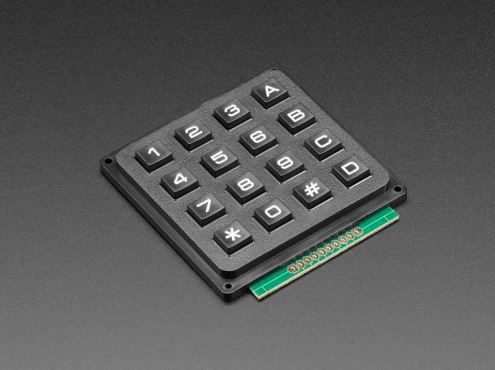
\includegraphics[scale=.8]{./Figures/keypad.JPG}
	\caption{Teclado matricial Adafruit 4x4.}
	\label{fig:keypad}
\end{figure}



\section{Comunicación CAN}
\label{comunicacion_can}

La implementación de una red CAN requiere consideraciones de diseño relacionadas con el \textit{bitrate} y los tiempos de bit con los cuales trabaja el protocolo para la lectura y envío de información. Como se explicó en la sección \ref{caracteristicas_can}, estas variables están relacionadas con la longitud del bus y con el ruido eléctrico al que está expuesto. En la figura \ref{tab:bit_times} se presentan los tiempos de bit recomendados para implementaciones de CANopen\citep{UnderstandingCAN}. Del listado se seleccionó la fila para un bus de 250 m, que recomienda un \textit{bitrate} de 250 kb/s. Estos parámetros se configuraron en el periférico CAN del microcontrolador.


\begin{table}[h]
	\centering
	\caption[Tiempos de bit recomendados para CANopen.]{Tiempos de bit recomendados para CANopen.}
	\begin{tabular}{c c c c c c}    
		\toprule
		\textbf{\textit{Bitrate}} & \textbf{Largo bus} & \textbf{Tiempo bit} & \textbf{\textit{Time quanta}} & \textbf{\textit{N quanta}} & \textbf{\textit{Sample}} \\
		\midrule
		1 Mb/s 		& 25 m 	& 1 $\mu$s		& 125 ns & 8 	& 6 \\
		800 kb/s 	& 50 m 	& 1.25 $\mu$s	& 125 ns & 10 	& 8 \\
		500 kb/s 	& 100 m & 2 $\mu$s		& 125 ns & 16 	& 14 \\
		250 kb/s 	& 250 m & 4 $\mu$s		& 250 ns & 16 	& 14 \\
		125 kb/s 	& 500 m & 8 $\mu$s		& 500 ns & 16 	& 14 \\
		50 kb/s 	& 1000 m & 20 $\mu$s	& 1.25 $\mu$s & 16 	& 14 \\
		20 kb/s 	& 2500 m & 50 $\mu$s	& 3.125 $\mu$s & 16 	& 14 \\
		10 kb/s 	& 5000 m & 100 $\mu$s	& 6.25 $\mu$s & 16 	& 14 \\
		\bottomrule
		\hline
	\end{tabular}
	\label{tab:bit_times}
\end{table}


La estructura empleada para la codificación de la información dentro de los mensajes CAN se muestra en la figura \ref{fig:estructura_mensajes}. Se utilizó tanto el campo de identificador estándar de 11 bits como los bytes de data para indicar el tipo de mensaje y la manera en que debe ser procesado.

Dentro del campo identificador se codificó la siguiente información:
\begin{itemize}
	\item Bit 1: Identificador de error
	\item Bits 2 a 10: \textit{Device ID}. Detalla el identificador único y fijo del dispositivo en la red.
	\item Bit 11: Dirección. Define si un mensaje es envíado por un dispositivo controlador de red (SCI-CAN) o un dispositivo periférico (SN-17).
\end{itemize}

Se estableció el primer bit del mensaje como identificación de errores para que  estos tengan la mayor prioridad en el proceso de arbitraje de la red CAN. Además, los mensajes que tienen este bit encendido no son filtrados por ningún dispositivo de la red.

En los bits que corresponden al \textit{device ID} también se especifican identificadores comunes para mensajes del tipo \textit{broadcast}. Estos permiten la transmisión de información a todos los nodos de la red.

\begin{figure}[htbp]
	\centering
	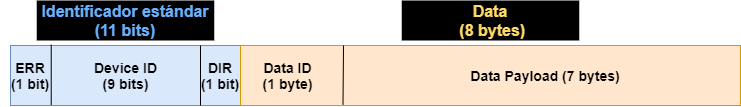
\includegraphics[scale=.5]{./Figures/estructura_mensaje.png}
	\caption{Estructura de mensajes CAN}
	\label{fig:estructura_mensajes}
\end{figure}

El campo de data tiene una longitud total de 8 bytes. Este contiene la siguiente información:
\begin{itemize}
	\item Byte 1: \textit{data ID}. Identifica el tipo de información del mensaje según la tabla \ref{tab:tipos_mensajes_CAN}
	\item Bytes 2 a 8: \textit{Data payload}. Contiene la información codificada según el \textit{data ID}.
\end{itemize}

La tabla \ref{tab:tipos_mensajes_CAN} presenta todos los \textit{data ID} implementados en el sistema. Para cada uno de estos tipos de mensaje la información se codifica de una forma diferente.

\begin{table}[h]
	\centering
	\caption[Operaciones SN-17]{Funciones de SN-17}
	\begin{tabular}{c c c}    
		\toprule
		\textbf{\textit{Data ID}} 	& \textbf{Tipo}  & \textbf{Descripción}\\
		\midrule
		Tipo de instrucción & Instrucción 	& Define la instrucción\\		
		Límite de torque 	& Instrucción	& Torque máximo de instrucción \\
		Modo de control		& Instrucción 	& Posición, velocidad, torque \\
		\textit{Set point}	& Instrucción 	& Valor de lazo de control \\
		\textit{Threshold}	& Instrucción 	& Valor de error admisible \\
		\textit{Hold time}	& Instrucción 	& Tiempo de cumplimiento \\
		\textit{Timeout}	& Instrucción 	& Tiempo de no cumplimiento \\
		Guardar posición	& Configuración & Guarda posición actual \\
		Calibrar posición	& Configuración & Guarda posición manual \\
		Constantes PID		& Configuración & Constantes lazo de control \\	
		Entradas y salidas	& Configuración & Funcionamiento de las IO \\
		\textit{Homing}		& Configuración & Establece rutina de cerado \\	
		Calibración			& Comando		& Inicia la rutina de calibración \\
		Activar motor		& Comando		& Enciende/apaga el motor \\		
		\textit{Go Home}	& Comando		& Inicia la rutina de cerado \\		
		Mover motor			& Comando		& Rota un ángulo específico\\
		Rotar motor			& Comando		& Gira a velocidad específica \\
		Torquear motor		& Comando		& Gira a torque específico \\
		Límite torque manual& Comando		& Limita el torque de comandos \\
		Activar salidas		& Comando		& Enciende/apaga salidas \\	
		Consultar motor		& Comando		& Consulta información del motor \\
		Programa manual		& Comando		& Corre un programa en modo maual \\
		Instrucción actual	& Supervisión	& Instrucción ejecutada del motor \\
		Encoder				& Supervisión	& Posición de encoder del motor \\
		Error				& Supervisión	& Tipo de error del motor \\
		Cambio de modo		& General		& Programación o operación \\
		\textit{Device ID}	& General		& Consulta de IDs de red \\
		\bottomrule
		\hline
	\end{tabular}
	\label{tab:tipos_mensajes_CAN}
\end{table}

Los tipos de mensajes implementados se dividen en:
\begin{itemize}
	\item Instrucción: Identifican los comandos en la secuencia de un programa en los sistemas SN-17 durante su operación. Son de lectura y escritura.
	\item Configuración: Establecen los parámetros operativos de los sistemas SN-17. Son de lectura y escritura.
	\item Comando: Indican a un sistema SN-17 una acción manual a realizar. Son de solo escritura.
	\item Supervisión: Indican al SCI-CAN el estado de un SN-17. Son de solo lectura.
	\item General: Son mensajes del tipo \textit{broadcast} para el control de la red. Son de lectura y escritura.
\end{itemize}

Los mensajes del tipo instrucción codifican un número según el \textit{data ID} que se utilice e identifican su posición en la secuencia del programa del sistema SN-17.

Los mensajes de configuración agregan información complementaria para indicar los parámetros modificables. Por ejemplo, en el caso de una constante PID, se indica en forma codificada cual es la constante y su valor. 

\section{Desarrollo de software}
\label{desarrollo_software}

\subsection{Arquitectura de Software}

El desarrollo del software se realizó sobre una placa de evaluación del microcontrolador seleccionado\citep{web_dev_board}. Esto permitió hacer pruebas del sistema previo al diseño del circuito y facilitó el proceso de implementación.

El software del sistema se diagramó siguiendo una estructura en capas. En la figura \ref{fig:arq_software} se muestra un esquema de la arquitectura implementada. Como se puede observar, las capas intermedias interactúan con la capa superior de aplicación mediante el uso de servicios públicos que cada uno de los manejadores ofrece. Las capas inferiores (Key, LCD I2C handler, buffer circular) no son visibles por la capa de aplicación, pero ofrecen funcionalidades para las capas intermedias. 

\begin{figure}[htbp]
	\centering
	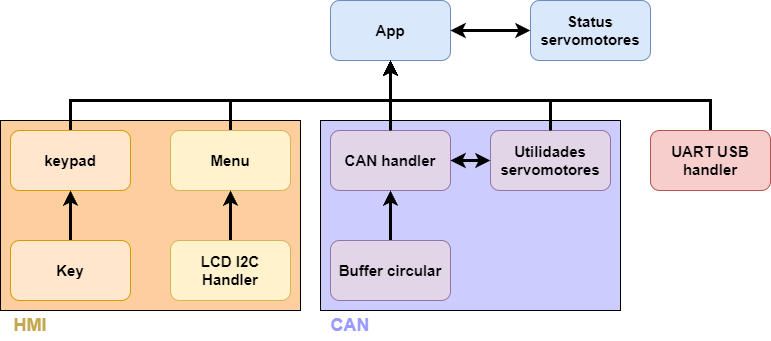
\includegraphics[scale=.5]{./Figures/arquitectura_software.png}
	\caption{Arquitectura de software}
	\label{fig:arq_software}
\end{figure}

La capa superior contiene a la aplicación que opera, en un mismo nivel, con una sección del código que almacena el estado de los distintos servomotores. En esta capa de software se coordina el funcionamiento e interacción de las capas intermedias.

El recuadro marcado como HMI (\textit{Human Machine Interface}) se relaciona con la sección del programa encargada de proveer la interfaz de usuario. Maneja las acciones del teclado matricial y la información que se visualiza en el display.

La sección CAN se relaciona con las configuraciones del periférico controlador del protocolo, las funciones para codificar los mensajes, el envío y recepción de mensajes y los servicios ofrecidos por los servomotores.

El manejador de UART-USB es el encargado de las interacciones con una PC. Realiza la codificación de información de los mensajes y procesa los datos recibidos por el puerto USB. 

En las subsecciones siguientes se explica el desarrollo de estos componentes principales de software.

\subsection{Driver CAN}

Para la implementación del módulo CAN handler de la figura \ref{fig:arq_software} se utilizó el periférico de este protocolo de comunicación en el microcontrolador seleccionado. Se realizó su configuración mediante la herramienta de desarrollo \textit{Microchip Studio} provista por el fabricante\citep{web_microchip_studio}, a través de la cual se seleccionaron:
\begin{itemize}
	\item Los tiempos de bit y la tasa de transmisión de 250 kb/s, según la figura \ref{fig:bit_times}.
	\item El uso del identificador estándar.
	\item El funcionamiento de los filtros.
	\item La opción de reenvío de mensaje en caso de colisiones.
\end{itemize}

El driver implementado opera por interrupción, con funciones de \textit{callback} llamadas cuando se recibe un mensaje o termina una transmisión. El software de este módulo resultó de una adaptación del código de ejemplo de operación del periférico CAN provisto por el fabricante.

En la figura \ref{fig:can_handler} se observa el flujo de programa implementado para el manejo de la recepción de los mensajes CAN.

\begin{figure}[htbp]
	\centering
	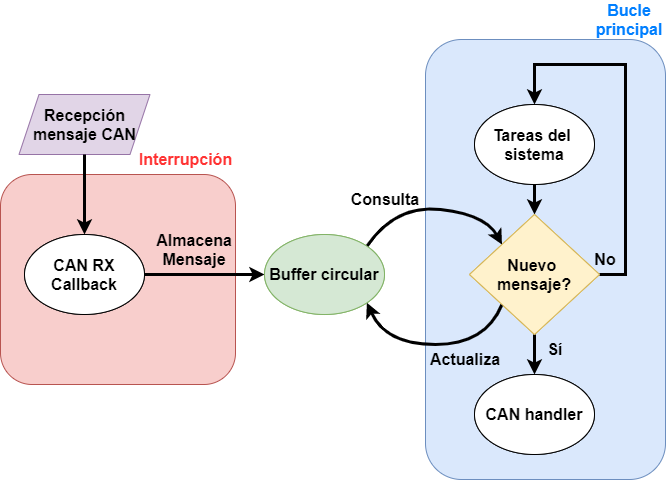
\includegraphics[scale=.5]{./Figures/Can_handler.png}
	\caption{Flujo de recepción de mensajes CAN.}
	\label{fig:can_handler}
\end{figure}

En la recepción de mensajes se empleó un módulo de software de \textit{buffer} circular\citep{tpf_gabriel}. La operación de recepción de mensajes CAN se hace en un estado de interrupción. Para evitar el procesamiento del mensaje en este estado se utiliza el algorítmo de \textit{buffer} circular, que almacena el mensaje en tiempo de interrupción sin procesarlo y señaliza esta condición. Estos mensajes son luego tratados dentro del bucle principal del programa. Este funcionamiento permite una operatoria ordenada y evita la pérdida de información en caso de que nuevos mensajes lleguen al bus sin que los anteriores hayan sido procesados.

Para la interpretación de los mensajes se construyó el módulo de software marcado como utilidades servomotores en la figura \ref{fig:arq_software}. Dentro de este se implementaron distintas funciones locales que decodifican el identificador y la data según el tipo de mensaje. Con el identificador CAN se determina si el mensaje recibido indica un error (primer bit) y si está dirigido a un SN-17 o al SCI-CAN (último bit de dirección). Con respecto a la información del tipo, como se explicó en la sección \ref{comunicacion_can}, se encuentra codificada en el primer byte de data del mensaje CAN. Esta información es discriminada por el algorítmo y, utilizando una estructura \textit{switch-case}, se selecciona la función decodificadora correspondiente.


\subsection{Interfaz HMI}

La interfaz HMI involucra la interacción del software del sistema con el teclado y con el display LCD. Su implementación implicó el desarrollo de los drivers de I2C para trabajar con la pantalla y manejadores para el teclado. También, se desarrolló un \textit{middleware} que controle un sistema de menúes, la interacción de ambos drivers y que ofrezca funcionalidades a la capa superior de aplicación.

La capa inferior del display se compone del driver I2C obtenido del fabricante del microcontrolador y una serie de servicios para mostrar información que son llamados por las capas superiores. Los servicios fueron modelados siguiendo ejemplos de código libre de implementaciones para Arduino\citep{web_repo_display_i2c}.

El driver del teclado sigue una arquitectura similar \citep{web_repo_keypad}. Este usó como ejemplo implementaciones libres de Arduino\citep{web_repo_keypad}. Esta capa ofrece servicios a las superiores para reconocer las teclas que fueron oprimidas.

Sobre estos manejadores se desarrolló un software que utiliza a ambos para generar el sistema de menúes y su interacción con un usuario. Mediante el uso del teclado se puede navegar a través de una lista de opciones que se muestran en el display y se permite visualizar y configurar los parámetros de los motores conectados. 

En la figura \ref{fig:menu} se muestra un ejemplo de cómo se presentan las opciones en el display. La flecha presente a la izquierda de la imagen es la que le permite al usuario ubicarse a medida que se navega por los menúes con la utilización del teclado.

\begin{figure}[htbp]
	\centering
	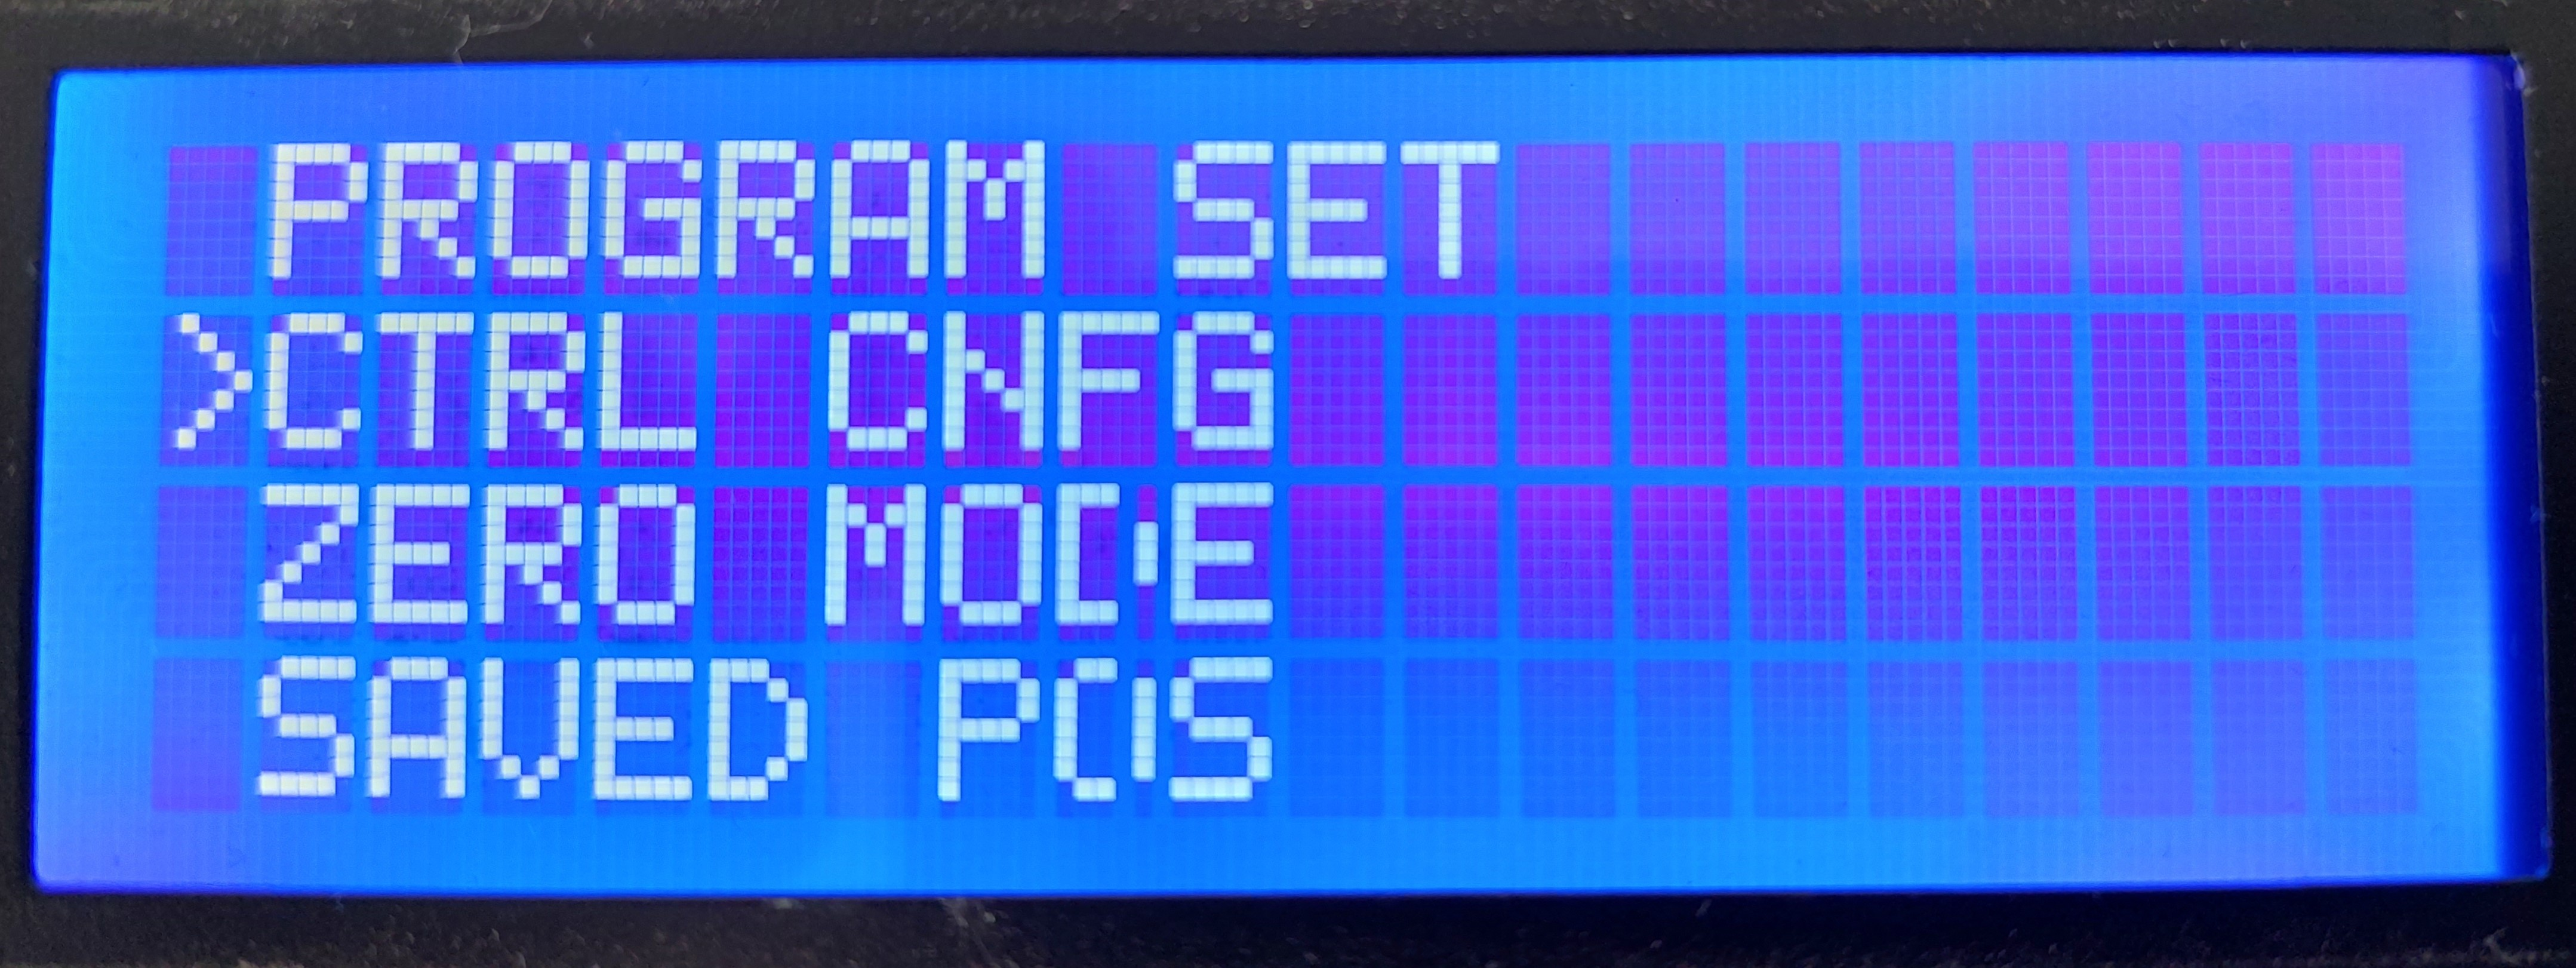
\includegraphics[scale=.08]{./Figures/display_menu.jpg}
	\caption{Ejemplo de opciones de menú}
	\label{fig:menu}
\end{figure}

Se planteó que el menú cuente con 2 pantallas diferentes según el estado en el que esté: monitoreo o programación. En el estado de monitoreo, se muestra una primera pantalla donde puede observarse el programa e instrucción que cada motor conectado está ejecutando en ese momento y puede navegarse para consultar la configuración, pero no puede ser modificada.

En el estado de programación, la configuración de los distintos motores es accesible para ser modificada y se muestran los distintos comandos manuales que pueden ejecutarse para cada motor. Al pasar del estado de monitoreo al de programación, la central envía un mensaje de \textit{broadcast} usando un ID prioritario a la red al que cada motor responde con su ID particular.

El software de menúes le indica a la capa superior de aplicación la acción solicitada por el usuario y es esta capa la que interactúa con los otros drivers, como se explicó en la sección \ref{desarrollo_software}.

\subsection{Interfaz UART-USB}

La interfaz UART-USB involucró el desarrollo de un manejador de UART desde el microcontrolador. La configuración de la comunicación se realizó con herramientas provistas por el fabricante. El software opera por interrupciones de hardware que llaman a funciones de \textit{callback} al completar una transmisión o recepción de un mensaje.

Los mensajes UART son adaptados a señales USB mediante el circuito integrado CY7C64225\citep{web_interfaz_USB_UART}. Esto permite la conexión del dispositivo con un monitor serial en una PC.

Sobre este manejador UART se construyó una herramienta de reporte que se ejecuta en la capa de aplicación que envía las acciones seleccionadas por el menú a través de USB. Esto permite confirmar que la información seleccionada es la correcta y facilita la detección de errores.

La interfaz de PC permite también configurar las acciones de los motores. La configuración una vez que llega al SCI-CAN es transformada en comandos CAN y enviada al nodo correspondiente.

\section{Modificaciones firmware SN-17}

Para que el sistema SCI-CAN pueda comunicarse con las plaquetas SN-17 ya instaladas se debió trabajar y actualizar su firmware. Estos cambios tuvieron 3 objetivos principales:
\begin{itemize}
	\item Incorporar los drivers de CAN y la estructura de mensajes planteada.
	\item Generar que las configuraciones y programas sean variables modificables.
	\item Lograr el almacenamiento de las configuraciones en memoria no volátil.
\end{itemize}

La implementación de CAN utilizó los mismos módulos de software desarrollados para el SCI-CAN sin modificaciones. Esto fue posible debido a que ambos sistemas utilizan el mismo microcontrolador. Siguiendo la estructura de CAN de la figura \ref{fig:arq_software}, los módulos de CAN handler y buffer circular se mantuvieron idénticos para ambos sistemas.

En la implementación del módulo de utilidades de servomotores se buscó también que ambos sistemas compartan el mismo software. Para ello, se planteó el uso de sentencias condicionales que determinen si un mensaje está dirigido a un sistema SCI-CAN o a un SN-17. A partir de esto se decide la acción a realizar en la capa de aplicación según la información del mensaje.

Para lograr que las configuraciones y los programas del sistema SN-17 sean modificables sin necesidad de cambiar el firmware se utilizó una estructura para almacenar la información. Esta es accedida directamente por la capa de aplicación, quien se encarga de administrarla. La información presente en la estructura se resume en la tabla \ref{tab:servo_status}.

\begin{table}[h]
	\centering
	\caption[Estructura de estado de servomotores.]{Estructura de estado de servomotores.}
	\begin{tabular}{c c}    
		\toprule
		\textbf{\textit{Nombre}}  & \textbf{Descripción}\\
		\midrule
		CAN ID  			& Identificador CAN							\\		
		Modo de trabajo		& Operación o configuración manual			\\
		Estado manual		& Estructura auxiliar para operación manual \\
		Control PID	 		& Información de variables de conttrol PID	\\
		Cerado				& Configuraciones de cerado de motor 		\\
		Posiciones memoria	& Memoria de posiciones guardadas	 		\\
		Encoder				& Última posición de encoder leída	 		\\
		Posición absoluta	& Última posición de eje calculada	 		\\
		Instrucción			& Instrucción actual en operación	 		\\
		Programa			& Programa actual en operación		 		\\
		Salidas				& Configuración de salidas discretas 		\\
		Entradas			& Configuración de entradas discretas 		\\
		Error				& Registro del último error			 		\\
		\bottomrule
		\hline
	\end{tabular}
	\label{tab:servo_status}
\end{table}

Esta misma estructura se replicó en el dispositivo SCI-CAN, donde se utilizan varias instancias, una por cada nodo conectado, donde se guarda el estado reportado por los sistemas SN-17. En el esquema de la figura \ref{fig:arq_software} el módulo Status servomotores es el que implementa la estructura descripta.

\section{Desarrollo de Hardware}
\label{desarrollo_hw}

El desarrollo del hardware se realizó con el software Altium Designer\citep{web_altium} y las placas fueron fabricadas por un proveedor habitual de Cambre ICyFSA\citep{web_pcbwing}. Para el diseño del PCB se tuvieron en cuenta las capacidades técnicas publicadas por el fabricante\citep{web_pcbwing_capabilities}.

Se establecieron las siguientes decisiones de diseño:
\begin{itemize}
	\item Placa de cuatro capas con dimensiones menores a 100 x 100 mm.
	\item Conectores COMBICON con tornillo\citep{web_combicon} para conexiones externas.
	\item Conectores XH\citep{web_xh_connector} para conexiones internas. 
\end{itemize} 

El primer paso del diseño fue determinar los subcircuitos del sistema. Estos son:
\begin{itemize}
	\item Microcontrolador.
	\item Regulador de tensión.
	\item Interfaz CAN.
	\item Entradas discretas.
	\item Salidas discretas.
	\item Interfaz UART-USB.
\end{itemize}

En cada uno de los subcircuitos se desarrolló un dibujo esquemático. En la figura \ref{fig:esquematico_can} se presenta el correspondiente a la interfaz CAN donde se muestra el \textit{transceiver} elegido y sus conexiones. Para cada uno de los componentes principales del sistema se siguieron las recomendaciones indicadas en su hoja de datos. 

\begin{figure}[htbp]
	\centering
	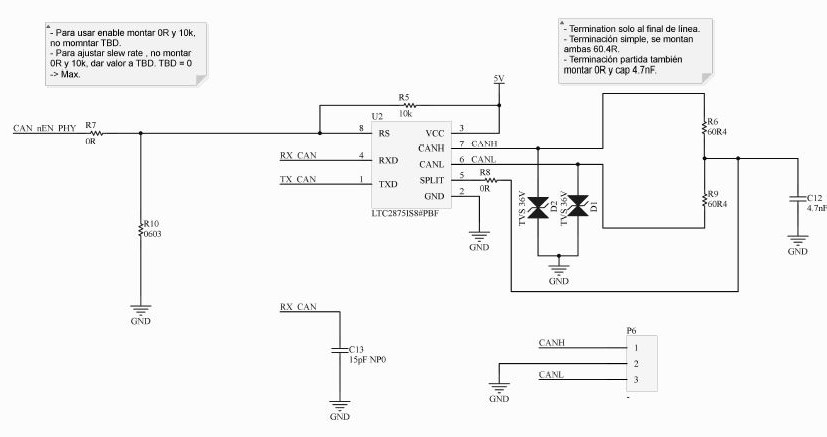
\includegraphics[scale=.7]{./Figures/sch_can.JPG}
	\caption{Esquemático de Interfaz CAN.}
	\label{fig:esquematico_can}
\end{figure}

Finalizados los subcircuitos esquemáticos, se continuó con el desarrollo del PCB. Primero, se determinaron las dimensiones de la plaqueta, manteniendo las restricciones impuestas y asegurando una cómoda posición de todos los componentes para permitir un ensamble manual. Se eligió una dimensión final de plaqueta de 100 x 80 mm. 

En el diseño del \textit{PCB} se buscó que:
\begin{itemize}
	\item Los subcircuitos quedaran separados.
	\item Los conectores se colocaran en los extremos de la plaqueta.
	\item Se respetara la aislación eléctrica de las entradas y salidas con el circuito de control.
	\item Se minimizara la longitud de las líneas de CAN y se maximizara su simetría.
\end{itemize}

La figura \ref{fig:render_pcb} muestra el render 3D del \textit{PCB} obtenido. En la parte superior se encuentran los circuitos de entradas y salidas industriales eléctricamente aislados por los optoacopladores y separados del resto del circuito. En la esquina inferior izquierda se encuentra el regulador de tensión de 5 V. En el centro el microcontrolador y a la derecha el circuito de CAN y de USB.

\begin{figure}[htbp]
	\centering
	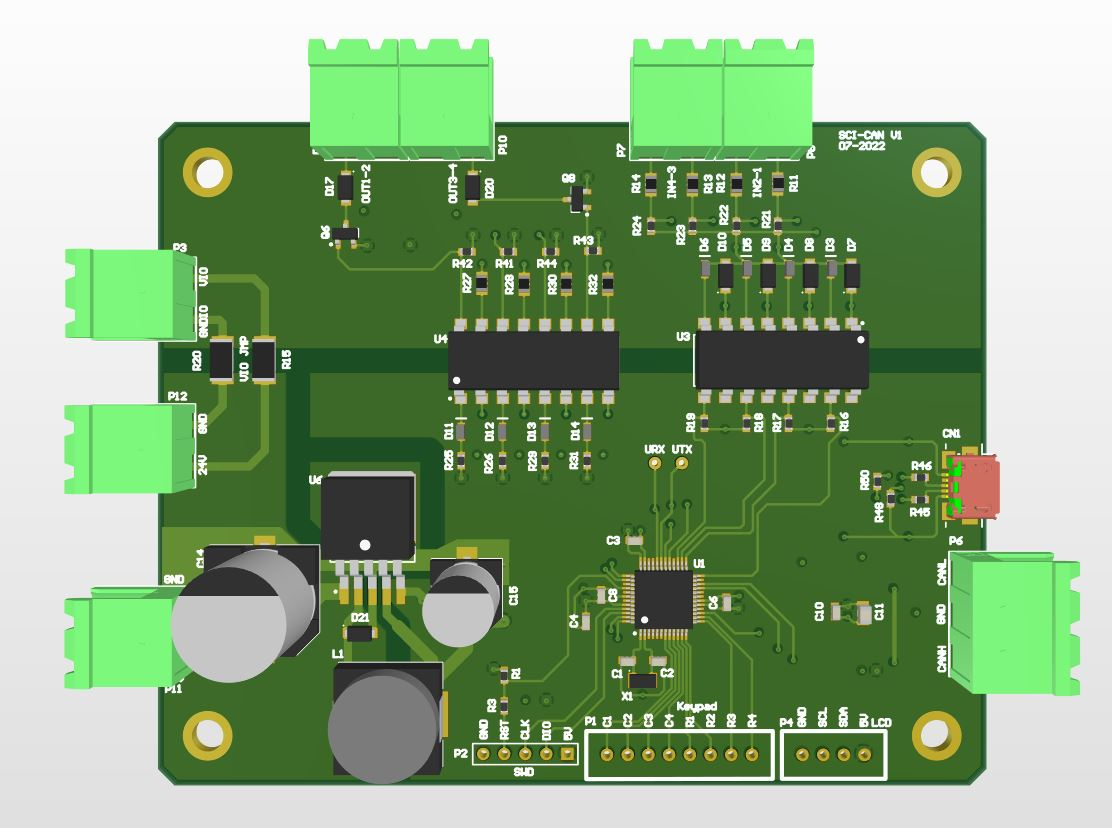
\includegraphics[scale=.4]{./Figures/pcb_sch.JPG}
	\caption{Render del \textit{PCB}.}
	\label{fig:render_pcb}
\end{figure}

\section{Desarrollo de gabinete}

El desarrollo del gabinete utilizó el software de diseño mecánico Autodesk Inventor\citep{web_inventor}. Se decidió armar un ensamble que incluya todos los componentes y que sea posible su impresión 3D.

Para los componentes adquiridos, como la pantalla LCD y la matriz de botones se tomaron los modelos 3D de uso libre de la plataforma GrabCAD\citep{web_grabcad}. Estos se verificaron para asegurarse que sus medidas correspondieran con el dispositivo físico adquirido. El modelo de la plaqueta electrónica SCI-CAN desarrollada se exportó desde el software Altium.

Una vez obtenidos los modelos de estos componentes, se realizó el desarrollo de las distintas piezas que conforman el gabinete. Como consideraciones de diseño se planteó:

\begin{itemize}
	\item Facilitar el acceso a los conectores de la plaqueta SCI-CAN.
	\item Proteger los circuitos internos de la plaqueta SCI-CAN.
	\item Presentar el teclado y el display de forma contigua.
	\item Esconder dentro del gabinete las conexiones entre el display y el teclado con la plaqueta SCI-CAN.
	\item Minimizar la cantidad de partes y de ajustes necesarios.
	\item Limitar los ajustes a roscas métricas.
\end{itemize}

Como restricción adicional de diseño se debió mantener las dimensiones máximas de las piezas a medidas menores que la capacidad de fabricación de la impresora 3D \textit{Creality Ender-3}\citep{web_ender3}. Esto corresponde a 220 x 220 x 250 mm.

En la figura \ref{fig:ensamble} se presenta una imagen del ensamble desarrollado tomada de Inventor. Es importante notar que las piezas superiores, donde están la pantalla y el teclado, se muestran transparentes para facilitar la visualización. El ensamble consta de 3 componentes: una tapa delantera donde apoyan el display y el teclado, una caja intermedia que encierra a estos y una caja trasera donde se coloca la plaqueta de control.

\begin{figure}[h!]
	\centering
	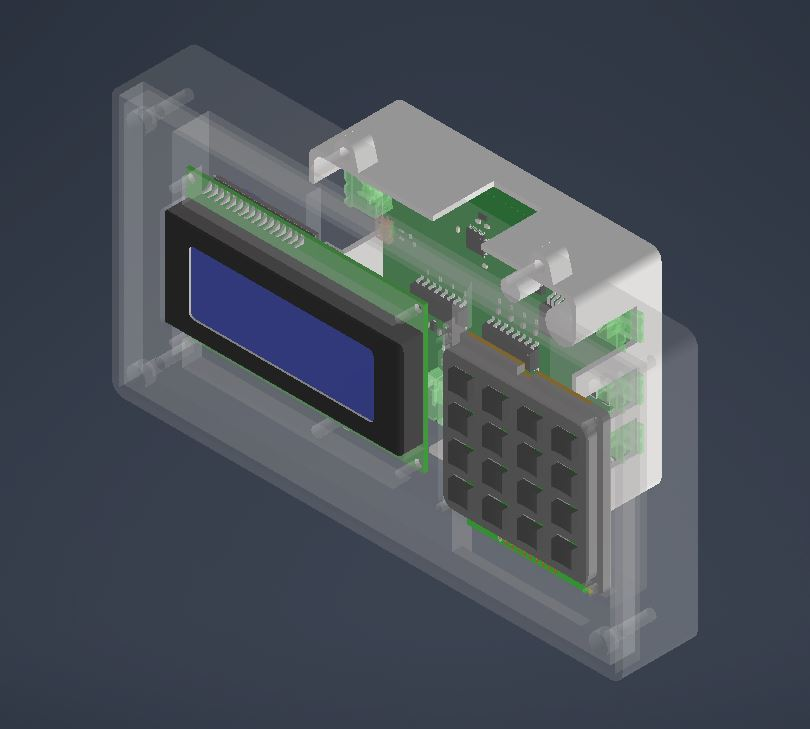
\includegraphics[scale=.6]{./Figures/asm_3d.JPG}
	\caption{Ensamble 3D de gabinete.}
	\label{fig:ensamble}
\end{figure}

\newpage

En la fabricación del conjunto se empleó el programa UltiMaker Cura\citep{web_cura3d} donde se generaron los archivos de fabricación para impresión 3D. Se decidió utilizar como material PLA, que es uno de los plásticos más económicos y simples de manipular y que cuenta con las características mecánicas apropiadas para la aplicación.
% Chapter Template

\chapter{Ensayos y resultados} % Main chapter title

\label{Chapter4} % Change X to a consecutive number; for referencing this chapter elsewhere, use \ref{ChapterX}

En este capítulo se detallan los ensayos y mediciones realizados sobre el sistema, para validar su funcionamiento y el cumplimiento de los requerimientos del trabajo. Se explicará cómo está compuesto el banco de pruebas utilizado y los instrumentos empleados, cómo se comprobó el envío de mensajes CAN a través de la red, qué ensayos eléctricos se realizaron sobre el sistema y cómo se verificó el envío de datos a través de UART y USB. Finalmente, se hablará de los ensayos que se realizaron en la planta de Cambre ICyFSA. 

%----------------------------------------------------------------------------------------
%	SECTION 1
%----------------------------------------------------------------------------------------

\section{Banco de pruebas}

Para validar el correcto funcionamiento del sistema, se ensambló un conjunto, se le cargó el firmware y se armó una red CAN con algunos motores paso a paso con plaquetas SN-17 conectadas. Dependiendo el ensayo a realizar, se conectaron 1 o más motores a la red, junto con un osciloscopio INSERTAR MARCA DEL OSCILOSCOPIO). Los dispositivos se alimentan con una fuente DC regulable YIHUA 305D\footnote{\url{http://yihuasoldering.com/product-4-2-30v-dc-power-supply/160008/}} trabajando a 24 V.

En la Figura \ref{fig:Banco} puede verse un esquema de la composición del banco de pruebas y los conexionados. En la PC se corre un programa de monitor serial llamado PuTTy\footnote{\url{https://www.putty.org/}} que se emplea para visualizar de forma simplificada el mensaje que el sistema intenta envíar a la red CAN.

\begin{figure}[htbp]
	\centering
	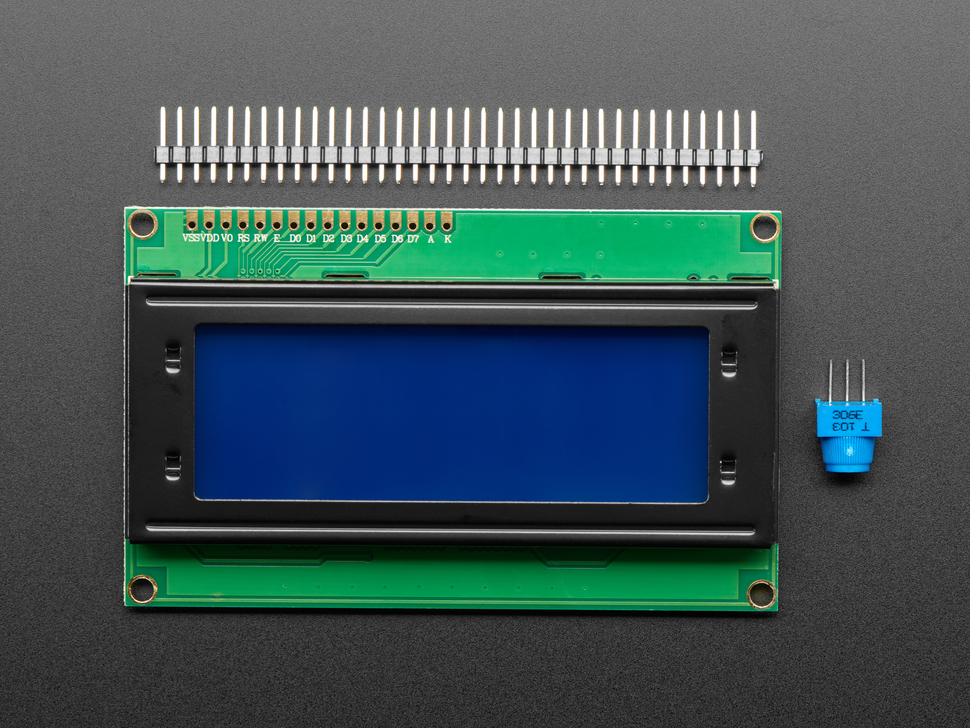
\includegraphics[scale=1]{./Figures/LCD.jpg}
	\caption{Banco de pruebas utilizado para verificaciones}
	\label{fig:Banco}
\end{figure}



\section{Ensayo de mensajes CAN}

En la Figura \ref{fig:niv_señal} se puede ver una de las tramas CAN tomadas desde el osciloscopio. En esta, se pueden ver claramente las señales CAN-H y CAN-L en un estado recesivo a 2.5 V y separándose un poco más de 1 V en ambos sentidos en un estado dominante, este es el comportamiento esperado. Notar también la falta de ruido en la señal, lo que indica la correcta operación de los resistores de terminación

\begin{figure}[htbp]
	\centering
	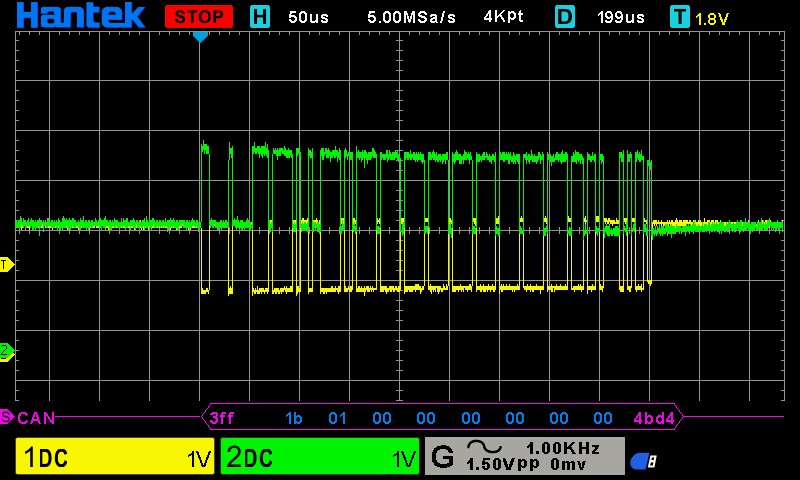
\includegraphics[scale=0.6]{./Figures/Message_Change_Operation_Mode_CONFIG.jpg}
	\caption{Níveles de señal CAN en osciloscopio}
	\label{fig:niv_señal}
\end{figure}

AGREGAR MEDICION DE TIEMPO

Para la verificación de los mensajes CAN se probaron cada uno de los mensajes posibles. Se revisó que el identificador y la data fueran correctas y que los sistemas conectados realizaran las acciones correspondientes.

En la Figura \ref{fig:mot_calib} se puede ver una imagen tomada del osciloscopio para la instrucción de calibrar motor (código: 0x0c). En la parte iferior puede verse el decodificador CAN que el osciloscopio trae incorporado, marcando correctamente la instrucción. También, se puede ver el identificador del mensaje (código: 0x0b) compuesto por el identificador del motor (0x05) y el bit final indicando que es un mensaje desde el dispositivo controlador. El resto de los bytes de data se marcan en 0, ya que no es necesario envíar más información para este tipo de mensaje, los últimos bytes pertenecen al CRC.

\begin{figure}[htbp]
	\centering
	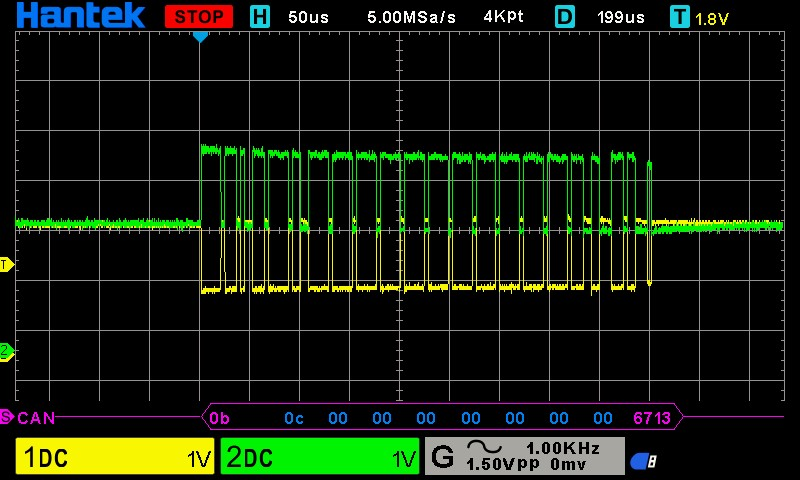
\includegraphics[scale=0.6]{./Figures/Motor_Calibrate.jpg}
	\caption{Instrucción calibrar motor}
	\label{fig:mot_calib}
\end{figure}

Otro ejemplo de mensaje puede visualizarse en la Figura \ref{fig:mot_move} en la que se envía al motor un comando manual de movimiento angular (código: 0x10), en dirección en contra de las agujas del reloj (código 0x01), un ángulo de 360 grados (códigos: 0x01 y 0x68). En este caso, como este ángulo es un número que requiere más de un byte para su representación, aparece descompuesto en el mensaje. Si se hace la conversión del número 168, de hexadecimal a decimal, se comprueba que es efectivamente 360. Al recibir el mensaje, el motor correctamente gira lo estipulado.

\begin{figure}[htbp]
	\centering
	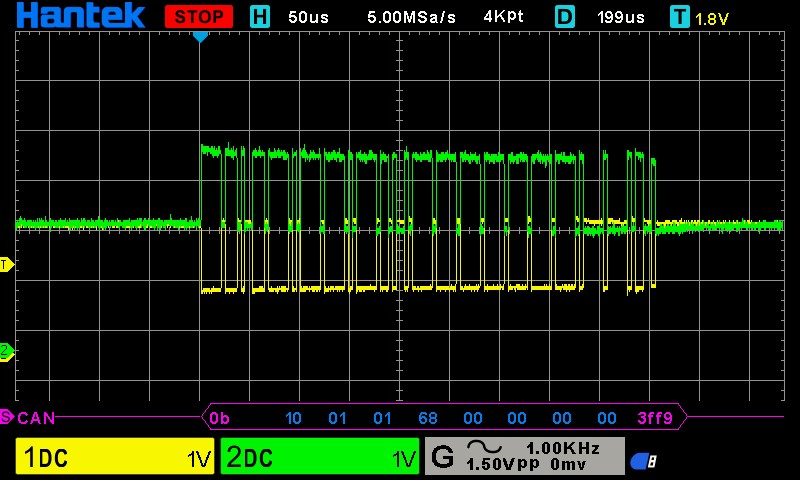
\includegraphics[scale=0.6]{./Figures/Motor_Manual_Move_CCW_360DEG.jpg}
	\caption{Instrucción manual mover motor}
	\label{fig:mot_move}
\end{figure}

\section{Ensayos eléctricos}

\section{Ensayos de mensajes UART}

\section{Pruebas de funcionamiento en planta}


% Chapter Template

\chapter{Conclusiones} % Main chapter title

\label{Chapter5} % Change X to a consecutive number; for referencing this chapter elsewhere, use \ref{ChapterX}


%----------------------------------------------------------------------------------------

%----------------------------------------------------------------------------------------
%	SECTION 1
%----------------------------------------------------------------------------------------

En este capítulo se hace un repaso de las actividades realizadas y se resume la conformidad de los requerimientos del trabajo con respecto a la planificación inicial. También, se hace mención a ciertos puntos a mejorar y a los próximos pasos del proyecto.

\section{Resultados obtenidos}

En general, el proyecto cumplió con todos los requerimientos planteados en la planificación. Se agregaron puntos adicionales, relacionados con la comunicación USB para facilitar el uso del dispositivo, que fueron implementados. Se considera que el objetivo del trabajo se logró de forma satisfactoria: el sistema obtenido facilitó la interacción con los sistemas SN-17 y permite monitorear el estado de los motores en operación.

Se destaca la manifestación de uno de los riesgos especificados en la planificación: el desabastecimiento de componentes electrónicos en el mercado mundial y la dificultad para traerlos a la Argentina generó retrasos en el desarrollo del proyecto e implicó la selección de componentes alternativos. El plan de mitigación de realizar las compras de forma prioritaria fue efectivo y permitió concluir el proyecto a tiempo.

Para el correcto desarrollo del trabajo, se utilizaron los conocimientos adquiridos a lo largo del posgrado, en particular:

\begin{itemize}
	\item Programación de microprocesadores: funcionamiento general de un microcontrolador, programación de periféricos (comunicación y timers) y máquinas de estado.
	\item Ingeniería de software: construcción de la arquitectura del software en capas, utilización de repositorios y definición de los servicios requeridos de cada uno de los drivers implementados.
	\item Protocolos de comunicación en sistemas embebidos: Utilización de diversos protocolos dentro del sistema, entre ellos, CAN, UART, SPI e I2C.
	\item Arquitectura de microprocesadores: Utilización de optimizaciones de compilador, cambios en linker script para almacenaje en memoria no volátil de información.
	\item Testing de software en sistemas embebidos: uso de herramientas de pruebas automáticas para encontrar errores en el software desarrollado.
	\item Diseño de circuitos impresos: recomendaciones para el desarrollo físico de la plaqueta. Utilización de reglas para desarrollo de PCB. Esquemáticos eléctricos separados por subcircuitos.
	\item Diseño para manufacturabilidad: selección de componentes para facilitar el ensamble, técnicas de soldadura recomendadas y consideraciones para ensamble automático.
\end{itemize}

Es importante notar que el sistema pudo ser montado y probado en una línea de montaje real en desarrollo en la planta industrial de Cambre ICyFSA. Los resultados de los ensayos realizados fueron satisfactorios.

%En la figura \ref{fig:au-0037} se muestra una imagen de la línea de ensamblaje en cuestión y se puede visualizar el sistema desarrollado junto con los actuadores que cuentan con los sistemas SN-17.
%
%\begin{figure}[htbp]
%	\centering
%	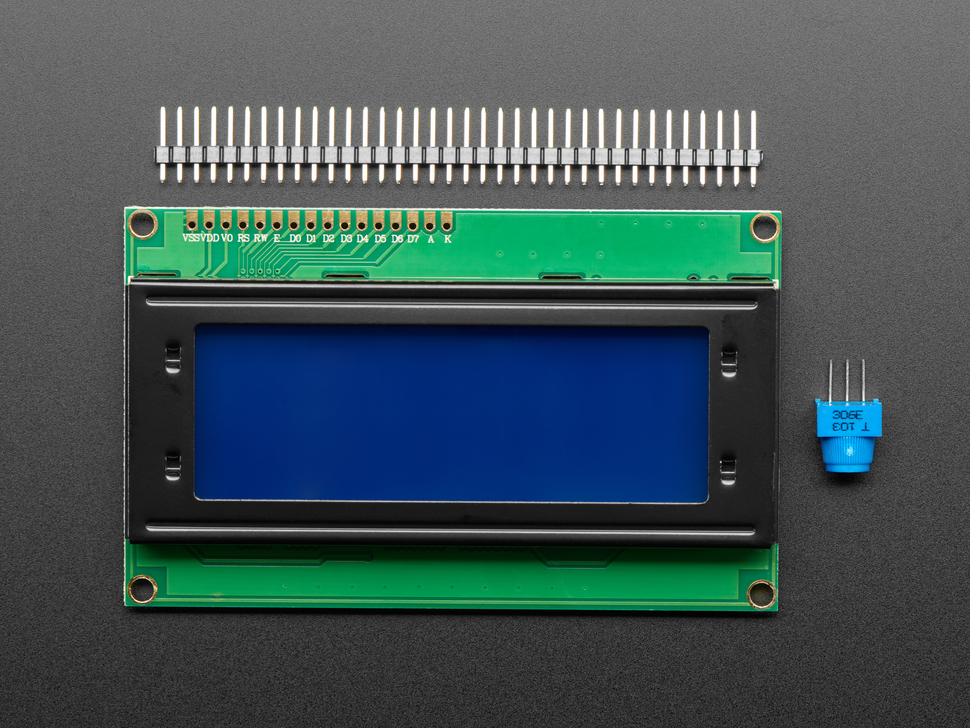
\includegraphics[scale=1]{./Figures/LCD.jpg}
%	\caption{Línea de ensamble automática con SCI-CAN - ARAMR FIGURA}
%	\label{fig:au-0037}
%\end{figure}

%----------------------------------------------------------------------------------------
%	SECTION 2
%----------------------------------------------------------------------------------------
\section{Próximos pasos}

Con el dispositivo implementado en las líneas productivas de Cambre ICyFSA, se le hará un seguimiento exhaustivo para corregir posibles errores y realizar posibles mejoras que puedan surgir con el uso del dispositivo. 

Se plantea como trabajo futuro:
\begin{itemize}
	\item Modificar el firmware para que trabaje con un sistema operativo, en lugar de \textit{bare metal}.
	\item Generar una interfaz gráfica para PC utilizando la conexión USB implementada.
	\item Implementar mensajes CAN entre diferentes dispositivos SN-17, sin la interacción del SCI-CAN para generar movimientos coordinados.
	\item Generar identificación dinámica de dispositivos, sin necesidad de utilizar identificadores de CAN fijos.
	\item Implementar otros protocolos de comunicación industriales, permitiendo más diversidad de interacciones.
\end{itemize}


%----------------------------------------------------------------------------------------
%	CONTENIDO DE LA MEMORIA  - APÉNDICES
%----------------------------------------------------------------------------------------

\appendix % indicativo para indicarle a LaTeX los siguientes "capítulos" son apéndices
% Incluir los apéndices de la memoria como archivos separadas desde la carpeta Appendices
% Descomentar las líneas a medida que se escriben los apéndices

%\include{Appendices/AppendixA}
%\include{Appendices/AppendixB}
%\include{Appendices/AppendixC}
%\include{Appendices/PlanProyecto.pdf}

%----------------------------------------------------------------------------------------
%	BIBLIOGRAPHY
%----------------------------------------------------------------------------------------

\Urlmuskip=0mu plus 1mu\relax
\raggedright
\printbibliography[heading=bibintoc]

%----------------------------------------------------------------------------------------

\end{document}